\subsection{DEFINITION OF AN ALGEBRA}

DEFINITION 1. Let A be a commutative ring. An algebra over A (or an A-algebra, or simply an algebra, when no confusion is to be feared) is a set E with a structure defined by giving the following:

\begin{enumerate}
\def\labelenumi{(\arabic{enumi})}
\item
  an A-module structure on E;
\item
  an A-bilinear mapping (II, § 3, no. 5) of \(\mathbf{E} \times \mathbf{E}\) into \(\mathbf{E}\) .
\end{enumerate}

The A-bilinear mapping of \(\mathbf{E} \times \mathbf{E}\) into \(\mathbf{E}\) occurring in this definition is called the multiplication of the algebra \(\mathbf{E}\) ; it is usually denoted by \((x, y) \mapsto x.y\) , or simply \((x, y) \mapsto xy\) .

Let \((\alpha_{i})_{i\in I}\) and \((\beta_{j})_{j\in J}\) be two families of elements of A, of finite support (I, § 2, no. 1). Then, for all families \((x_{i})_{i\in I}\) and \((y_{j})_{j\in J}\) of elements of E, the general distributivity formula (I, § 3, no. 4)

\[
\left(\sum_ {i \in I} \alpha_ {i} x _ {i}\right) \left(\sum_ {j \in J} \beta_ {j} y _ {j}\right) = \sum_ {(i, j) \in I \times J} \left(\alpha_ {i} \beta_ {j}\right) \left(x _ {i} y _ {j}\right)\tag{1}
\]

holds; in particular

\[
(\alpha x) y = x (\alpha y) = \alpha (x y) \quad \text { for } \alpha \in \mathrm{A}, x \in \mathrm{E} \text { and } y \in \mathrm{E}.\tag{2}
\]

The bilinear mapping \((x,y)\mapsto yx\) of E × E into E and the A-module structure on E define an A-algebra structure on E, called opposite to the given algebra structure. The set E with this new structure is called the opposite algebra to the algebra E; it is often denoted by \(E^{0}\) . The A-algebra E is called commutative if it is identical with its opposite, in other words if multiplication in E is commutative. An isomorphism of E onto \(E^{0}\) is also called an anti-automorphism of the algebra E.

When multiplication in the algebra E is associative, E is called an associative A-algebra. When multiplication in E admits an identity element (necessarily unique (I, §2, no. 1)), this element is called the unit element of E and E is called a unital algebra.

Examples. (1) Every commutative ring A can be considered as an (associative and commutative) A-algebra.

\begin{enumerate}
\def\labelenumi{(\arabic{enumi})}
\setcounter{enumi}{1}
\item
  Let E be a pseudo-ring (I, §8, no. 1). Multiplication on E and the unique Z-module structure on E define on E an associative Z-algebra structure.
\item
  Let \(\mathbf{F}\) be a set and \(\mathbf{A}\) a commutative ring. The set \(\mathbf{A}^{\mathbf{F}}\) of all mappings of \(\mathbf{F}\) into \(\mathbf{A}\) , with the product ring structure (I, § 8, no. 10) and the product
\end{enumerate}

A-module structure (II, §1, no. 5) is an associative and commutative A-algebra.

\begin{enumerate}
\def\labelenumi{(\arabic{enumi})}
\setcounter{enumi}{3}
\tightlist
\item
  Let E be an A-algebra; the internal laws \((x,y)\mapsto xy+yx\) and \((x,y)\mapsto xy-yx\) define (with the A-module structure on E) two A-algebra structures on E, which are not in general associative; the first law
\end{enumerate}

\[
(x, y) \mapsto x y + y x
\]

is always commutative.

DEFINITION 2. Given two algebras E, E' over a commutative ring A, a homomorphism of E into E' is a mapping \(f: \mathbf{E} \to \mathbf{E}'\) such that

\begin{enumerate}
\def\labelenumi{(\arabic{enumi})}
\item
  \(f\) is an A-module homomorphism;
\item
  \(f(xy) = f(x)f(y)\) for all \(x \in \mathbf{E}\) and \(y \in \mathbf{E}\) .
\end{enumerate}

Clearly the composition of two A-algebra homomorphisms is an A-algebra homomorphism. Every bijective algebra homomorphism is an isomorphism. Therefore A-algebra homomorphisms may be taken as morphisms of the species of A-algebra structure (Set Theory, IV, 2, no. 1). We shall always suppose in what follows that this choice of morphisms has been made. If E, E' are two A-algebras, let \(\operatorname{Hom}_{\mathbf{A}-\operatorname{alg}}(\mathbf{E}, \mathbf{E}')\) denote the set of A-algebra homomorphisms of E into E'.

Let E, E' be two algebras each with a unit element. A homomorphism of E into E' mapping the unit element of E to the unit element of E' is called a unital homomorphism (or unital algebra morphism).

\subsection{SUBALGEBRAS. IDEALS. QUOTIENT ALGEBRAS}

Let A be a commutative ring and E an A-algebra. If F is a sub-A-module of W which is stable under the multiplication on E, the restriction to \(F \times F\) of the multiplication of E defines (with the A-module structure on F) an A-algebra structure on F. F, with this structure, is called a subalgebra of the A-algebra E. Every intersection of subalgebras of E is a subalgebra of E. For every family \((x_{i})_{i \in I}\) of elements of E, the intersection of the subalgebras of E containing all the \(x_{i}\) is called the subalgebra of E generated by the family \((x_{i})_{i \in I}\) and \((x_{i})_{i \in I}\) is called a generating system (or generating family) of this subalgebra. If \(u: E \to E'\) is an A-algebra homomorphism, the image \(u(F)\) of every subalgebra F of E is a subalgebra of \(E'\) .

Let E be an associative algebra. For every subset M of E, the set M' of elements of E which are permutable with all the elements of M is a subalgebra of E called the centralizer subalgebra of M in E (I, § 1, no. 5). The centralizer M'' of M' in E is also called the bicentralizer of M; clearly M ⊆ M''. It follows that M' is contained in its bicentralizer M'', which is just the centralizer of M''; but the relation M ⊆ M'' implies M'' ⊆ M', so that M' = M'' (cf.~Set Theory, III, § 1, no. 7, Proposition 2). If F is a subalgebra of E, the centre of F is the intersection F ∩ F' of F and its centralizer F' in E. Note that if

F is commutative, then \(F \subset F'\) and hence \(F' \supset F''\) ; the bicentralizer \(F''\) of F is in this case the centre of F.

For certain non-associative algebras (for example Lie algebras) the notions of centralizer of a subalgebra and centre are defined differently (Lie Groups and Lie algebras, I, § 1, no. 6).

A subset \(\mathfrak{a}\) of an A-algebra \(\mathbf{E}\) is called a left ideal (resp. right ideal) of \(\mathbf{E}\) when \(\mathfrak{a}\) is a sub-A-module of \(\mathbf{E}\) and the relations \(x \in \mathfrak{a}, y \in \mathbf{E}\) imply \(yx \in \mathfrak{a}\) (resp. \(xy \in \mathfrak{a}\) ). It amounts to the same to say that \(\mathfrak{a}\) is a left ideal of \(\mathbf{E}\) or a right ideal of the opposite algebra \(\mathbf{E}^0\) . A two-sided ideal of \(\mathbf{E}\) is a subset \(\mathfrak{a}\) of \(\mathbf{E}\) which is both a left ideal and a right ideal. When \(\mathbf{E}\) is associative and admits a unit element \(e\) , then, for \(\alpha \in \mathbf{A}\) and \(x \in \mathbf{E}\) , \(\alpha x = (\alpha e)x = x(\alpha e)\) by virtue of (2) (no. 1) and hence the (right, left, two-sided) ideals of the ring \(\mathbf{E}\) (I, §8, no. 6) are identical with the (right, left, two-sided) ideals of the algebra \(\mathbf{E}\) . Every sum and every intersection of left (resp. right, two-sided) ideals of the algebra \(\mathbf{E}\) is a left (resp. right, two-sided) ideal. The intersection of the left (resp. right, resp. two-sided) ideals containing a subset \(\mathbf{X}\) of \(\mathbf{E}\) is called the left (resp. right, resp. two-sided) ideal of \(\mathbf{E}\) generated by \(\mathbf{X}\) .

Let \(\mathfrak{b}\) be a two-sided ideal of an A-algebra E. If \(x \equiv x'\pmod{\mathfrak{b}}\) and \(y \equiv y'\pmod{\mathfrak{b}}\) , then

\[
x (y - y ^ {\prime}) \in \mathfrak {b} \quad \text { and } \quad (x - x ^ {\prime}) y ^ {\prime} \in \mathfrak {b}
\]

and hence \(xy \equiv x'y' \pmod{b}\) . Hence an internal law can be defined on the quotient A-module E/b, which is the quotient of the multiplication law \((x,y) \mapsto xy\) of E by the equivalence relation \(x \equiv x' \pmod{b}\) (I, § 1, no. 6). It is immediately verified that this quotient law is an A-bilinear mapping of \((\mathrm{E} / \mathfrak{b}) \times (\mathrm{E} / \mathfrak{b})\) into E/b; it therefore defines with the A-module structure on E/b an A-algebra structure on E/b. E/b, with this algebra structure, is called the quotient algebra of the algebra E by the two-sided ideal b. The canonical mapping \(p: \mathrm{E} \to \mathrm{E} / \mathfrak{b}\) is an algebra homomorphism.

Let E, E' be two A-algebras and \(u:E \rightarrow E'\) an algebra homomorphism. The image \(u(\mathbf{E})\) is a subalgebra of \(E'\) and the kernel \(b = u(0)\) is a two-sided ideal of E; further, in the canonical decomposition of u:

\[
\mathrm{E} \xrightarrow {p} \mathrm{E} / \mathfrak {b} \xrightarrow {v} u (\mathrm{E}) \xrightarrow {j} \mathrm{E} ^ {\prime}
\]

v is an algebra isomorphism. More generally, all the results of Chapter I, § 8, no. 9 are still valid (and also their proofs) when the word ``ring'' is replaced by ``algebra''.

Let A be a commutative ring and E an A-algebra. On the set \(\tilde{\mathbf{E}} = \mathbf{A} \times \mathbf{E}\) , we define the following laws of composition:

\[
\begin{array}{r} (\lambda , x) + (\mu , y) = (\lambda + \mu , x + y) \\ (\lambda , x) (\mu , y) = (\lambda \mu , x y + \mu x + \lambda y) \\ \lambda (\mu , x) = (\lambda \mu , \lambda x). \end{array}
\]

It is immediately verified that \(\tilde{E}\) , with these laws of composition, is an algebra over A and \((1,0)\) is a unit element of this algebra. The set \(\{0\}\times E\) is a two-sided ideal of \(\tilde{E}\) and \(x\mapsto(0,x)\) is an isomorphism of the algebra E onto the subalgebra \(\{0\}\times E\) , by means of which E and \(\{0\}\times E\) are identified. \(\tilde{E}\) is called the algebra derived from E by adjoining a unit element; it is associative (resp. commutative) if and only if E is.

\subsection{DIAGRAMS EXPRESSING ASSOCIATIVITY AND COMMUTATIVITY}

Let A be a commutative ring and E an A-module; being given a bilinear mapping of \(E \times E\) into E is equivalent to being given an A-linear mapping:

\[
m: \mathbf {E} \otimes_ {\mathbf {A}} \mathbf {E} \rightarrow \mathbf {E}
\]

(II, §3, no. 5). An A-algebra structure on E is therefore defined by giving an A-module structure on E and an A-linear mapping of E \(\otimes_{\mathbf{A}}\) E into E.

Let \(E'\) be another A-algebra and \(m': E' \otimes_{A} E' \to E'\) the A-linear mapping defining the multiplication of \(E'\) . A mapping \(f: E \to E'\) is an A-algebra homomorphism if and only if \(f\) is a mapping rendering commutative the diagram

\[
\begin{array}{c} \mathrm{E} \otimes_ {\mathrm{A}} \mathrm{E} \xrightarrow {f \otimes f} \mathrm{E} ^ {\prime} \otimes_ {\mathrm{A}} \mathrm{E} ^ {\prime} \\ m \Biggl \downarrow \\ \mathrm{E} \xrightarrow {f} \mathrm{E} ^ {\prime} \end{array}
\]

For an A-algebra E to be associative, it is necessary and sufficient (taking account of the associativity of tensor products, cf.~II, § 3, no. 8) that the diagram of A-linear mappings

\[
\begin{array}{c} \mathrm{E} \otimes_ {\mathrm{A}} \mathrm{E} \otimes_ {\mathrm{A}} \mathrm{E} \xrightarrow {m \otimes 1 _ {\mathrm{E}}} \mathrm{E} \otimes_ {\mathrm{A}} \mathrm{E} \\ \downarrow^ {1 _ {\mathrm{E}} \otimes m} \\ \mathrm{E} \otimes_ {\mathrm{A}} \mathrm{E} \xrightarrow {m} \mathrm{E} \end{array}
\]

be commutative. Similarly, for the A-algebra E to be commutative, it is necessary and sufficient that the diagram of A-linear mappings

\[
\begin{array}{c} \mathrm{E} \otimes_ {\mathrm{A}} \mathrm{E} \xrightarrow {\sigma} \mathrm{E} \otimes_ {\mathrm{A}} \mathrm{E} \\ \Biggl \downarrow m \Biggl \downarrow m \\ \mathrm{E} \end{array}
\]

be commutative, where \(\sigma\) denotes the canonical A-linear mapping defined by \(\sigma(x \otimes y) = y \otimes x\) for \(x \in \mathbf{E}\) , \(y \in \mathbf{E}\) (II, § 3, no. 1, Corollary 2 to Proposition 1).

For all \(c \in \mathbf{E}\) , let \(\eta_c\) denote the A-linear mapping of \(\mathbf{A}\) into \(\mathbf{E}\) defined by the condition \(\eta_c(1) = c\) . For \(c\) to be a unit element of \(\mathbf{E}\) , it is necessary and sufficient that the two diagrams

\pandocbounded{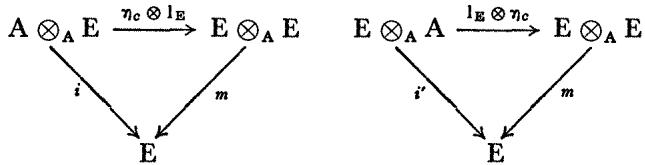
\includegraphics[keepaspectratio]{images/part003_ee0531f1.jpg}}

be commutative (i and i' denoting the canonical isomorphisms (II, §3, no. 4, Proposition 4)).

Let E be an A-algebra with unit element e and let \(\eta = \eta_{e}\) (also denoted by \(\eta_{E}\) ); then \(\eta(\alpha\beta) = \eta(\alpha)\eta(\beta) = \alpha\eta(\beta)\) , for by (2) (no. 1),

\[
(\alpha e) (\beta e) = (\alpha \beta) e = \alpha (\beta e);
\]

hence \(\eta\) is an A-algebra homomorphism. Observe that the A-module structure on E can be defined using \(\eta\) , for

\[
\alpha x = \eta (\alpha). x \quad \text { for } \alpha \in \mathrm{A}, x \in \mathrm{E}\tag{3}
\]

(where, on the right hand side, multiplication is in E). The image of the homomorphism \(\eta\) is a subalgebra of E whose elements commute with all those of E. The kernel of the homomorphism \(\eta\) is the annihilator of the element \(e\) of the A-module E; by (3), it is also the annihilator of the A-module E (II, § 1, no. 12).

When the algebra E is unital and associative, \(\eta\) is a ring homomorphism. Conversely, let \(\rho:A\to B\) be a ring homomorphism such that the image \(\rho(A)\) is contained in the centre of B, assuming also that the ring A is commutative; then an A-algebra structure is defined on B which is associative and unital, by writing (cf.~(3))

\[
\lambda x = \rho (\lambda). x \quad \text { for } \lambda \in \mathbf {A}, x \in \mathbf {E}.
\]

\subsection{PRODUCTS OF ALGEBRAS}

Let \((\mathbf{E}_i)_{i\in I}\) be a family of algebras over the same commutative ring A. It is immediately verified that on the product set \(\mathbf{E} = \prod_{i\in I}\mathbf{E}_i\) , the product A-module structure (II, § 1, no. 5) and the multiplication

\[
\left(\left(x _ {i}\right), \left(y _ {i}\right)\right) \mapsto \left(x _ {i} y _ {i}\right)\tag{4}
\]

define an A-algebra structure; with this structure, the set E is called the product algebra of the family of algebras \((\mathbf{E}_{i})_{i\in I}\) .

When all the algebras \(E_{t}\) are associative (resp. commutative, resp. unital), so is their product. Moreover, all the properties stated in I, §8, no. 10, extend without modification to arbitrary products of algebras.

\subsection{RESTRICTION AND EXTENSION OF SCALARS}

Let \(A_{0}\) and A be two commutative rings and \(\rho:A_{0}\to A\) a ring homomorphism. If E is an A-algebra, we denote (conforming with II, § 1, no. 13) by \(\rho_{*}(E)\) the \(A_{0}\) -module defined by addition on E and the external law

\[
\lambda . x = \rho (\lambda) x \quad \text { for   all } \lambda \in A _ {0} \text { and   all } x \in E.
\]

Multiplication in E and the \(A_{0}\) -module structure on \(\rho_{*}(E)\) define an \(A_{0}\) -algebra structure on \(\rho_{*}(E)\) . When \(A_{0}\) is a subring of A and \(\rho\) the canonical injection, the algebra \(\rho_{*}(E)\) is said to be obtained from E by restricting the ring A of scalars to \(A_{0}\) . By an abuse of language, this is also sometimes said when \(\rho\) is arbitrary.

Let F be an \(A_{0}\) -algebra. An \(A_{0}\) -algebra homomorphism \(F \to \rho_{*}(E)\) is called a semi-homomorphism (relative to \(\rho\) ) or a \(\rho\) -homomorphism of F into the A-algebra E; it is also called an \(A_{0}\) -homomorphism if no confusion arises. If E, \(E'\) are two A-algebras, every A-algebra homomorphism \(E \to E'\) is also an \(A_{0}\) -algebra homomorphism \(\rho_{*}(E) \to \rho_{*}(E')\) .

Consider now two commutative rings A and B and a ring homomorphism \(\rho: \mathbf{A} \to \mathbf{B}\) . For every A-module E, the B-module \(\rho^{*}(\mathbf{E}) = \mathbf{E} \otimes_{\mathbf{A}} \mathbf{B}\) , obtained from E by extending the ring A of scalars to B, has been defined (II, § 5, no. 1). If E is also an A-algebra, we shall define on \(\rho^{*}(\mathbf{E})\) a B-algebra structure. For this, observe that \((\mathbf{E} \otimes_{\mathbf{A}} \mathbf{B}) \otimes_{\mathbf{B}} (\mathbf{E} \otimes_{\mathbf{A}} \mathbf{B})\) is canonically isomorphic to \((\mathbf{E} \otimes_{\mathbf{A}} \mathbf{E}) \otimes_{\mathbf{A}} \mathbf{B}\) (II, § 5, no. 1, Proposition 3). If \(m: \mathbf{E} \otimes_{\mathbf{A}} \mathbf{E} \to \mathbf{E}\) defines the multiplication on E, the mapping \(m \otimes l_{\mathbf{B}}: (\mathbf{E} \otimes_{\mathbf{A}} \mathbf{E}) \otimes_{\mathbf{A}} \mathbf{B} \to \mathbf{E} \otimes_{\mathbf{A}} \mathbf{B}\) is therefore canonically identified with a B-linear mapping

\[
m ^ {\prime}: \rho^ {*} (\mathbf {E}) \otimes_ {\mathbf {B}} \rho^ {*} (\mathbf {E}) \rightarrow \rho^ {*} (\mathbf {E})
\]

which defines the desired B-algebra structure on \(\rho^{*}(\mathbf{E})\) . Hence

\[
(x \otimes \beta) (x ^ {\prime} \otimes \beta^ {\prime}) = (x x ^ {\prime}) \otimes (\beta \beta^ {\prime})\tag{5}
\]

for \(x, x'\) in \(\mathbf{E}\) , \(\beta\) and \(\beta'\) in \(\mathbf{B}\) . The B-algebra \(\rho^*(\mathbf{E})\) is said to be derived from the A-algebra \(\mathbf{E}\) by extending the ring \(\mathbf{A}\) of scalars to \(\mathbf{B}\) (by means of \(\rho\) ). It is also denoted by \(\mathrm{E}_{(\mathbf{B})}\) or \(\mathbf{E} \otimes_{\mathbf{A}} \mathbf{B}\) . When \(\mathbf{E}\) is associative (resp. commutative, resp. unital), so is \(\rho^*(\mathbf{E})\) .

PROPOSITION 1. For every A-algebra E, the canonical mapping \(\phi_{\mathbf{E}}: x \mapsto x \otimes 1\) of E into \(\mathrm{E}_{(\mathbf{B})}\) is an A-homomorphism of algebras. Moreover, for every B-algebra F and every A-homomorphism \(f: \mathbf{E} \to \mathbf{F}\) , there exists one and only one B-homomorphism \(\bar{f}: \mathbf{E}_{(\mathbf{B})} \to \mathbf{F}\) such that \(\bar{f}(x \otimes 1) = f(x)\) for all \(x \in \mathbf{E}\) .

The first assertion follows immediately from the definition of multiplication in \(\mathrm{E}_{(\mathrm{B})}\) , which gives \((x\otimes1)(x'\otimes1)=(xx')\otimes1\) for \(x\in E\) and \(x'\in E\) . The existence and uniqueness of the B-linear mapping \(\bar{f}\) of \(\mathrm{E}_{(\mathrm{B})}\) into F satisfying the relation \(\bar{f}(x\otimes1)=f(x)\) for all \(x\in E\) follow from II, §5, no. 1, Proposition 1; here it all amounts to verifying that \(\bar{f}(yy')=\bar{f}(y)\bar{f}(y')\) for y and \(y'\) in \(\mathrm{E}_{(\mathrm{B})}\) ; as the elements of the form \(x\otimes1\) (with \(x\in E\) ) generate the B-module \(\mathrm{E}_{(\mathrm{B})}\) , attention may be confined to the case where \(y=x\otimes1\) , \(y'=x'\otimes1\) with \(x\in E\) , \(x'\in E\) ; as \(yy'=(xx')\otimes1\) , the relation \(\bar{f}(yy')=\bar{f}(y)\bar{f}(y')\) then follows from \(f(xx')=f(x)f(x')\) .

It can also be said that \(f \mapsto \bar{f}\) is a canonical bijection

\[
\operatorname{Hom} _ {\mathrm{A-alg.}} (\mathrm{E}, \rho_ {*} (\mathrm{F})) \rightarrow \operatorname{Hom} _ {\mathrm{B-alg.}} (\rho^ {*} (\mathrm{E}), \mathrm{F}).\tag{6}
\]

The ordered pair consisting of \(E_{(B)}\) and \(\phi_{E}\) is therefore a solution of the universal mapping problem (Set Theory, IV, §3, no. 1) where \(\Sigma\) is the species of B-algebra structure and the \(\alpha\) -mappings the A-homomorphisms from E to a B-algebra.

COROLLARY. Let E, E' be two A-algebras; for every A-homomorphism of algebras \(u: E \to E'\) , \(u \otimes l_{B}\) is the unique B-homomorphism of algebras v: \(E \otimes_{A} B \to E' \otimes_{A} B\) rendering commutative the diagram

\[
\begin{array}{c} \mathrm{E} \xrightarrow {\phi_ {\mathrm{E}}} \mathrm{E} \otimes_ {\mathrm{A}} \mathrm{B} \\ u \Biggl \downarrow \\ \mathrm{E} ^ {\prime} \xrightarrow [ \phi_ {\mathrm{E} ^ {\prime}} ]{} \mathrm{E} ^ {\prime} \otimes_ {\mathrm{A}} \mathrm{B} \end{array}
\]

Let C be a third commutative ring and \(\sigma: B \to C\) a ring homomorphism; it is immediate that the canonical C-homomorphism

\[
\sigma^ {*} (\rho^ {*} (\mathbf {E})) \rightarrow (\sigma \circ \rho) ^ {*} (\mathbf {E})
\]

mapping \((x\otimes 1)\otimes 1\) to \(x\otimes 1\) for all \(x\in \mathbf{E}\) (II, §5, no. 1, Proposition 2) is an algebra isomorphism.

\subsection{INVERSE AND DIRECT LIMITS OF ALGEBRAS}

Let I be a preordered set and \((\mathbf{A}_{i},\phi_{ij})\) an inverse system of commutative rings with I as indexing set. Let \((\mathbf{E}_{i},f_{ij})\) be an inverse system of \(A_{i}\) -modules with I as indexing set (II, §6, no. 1) and suppose further that each \(E_{i}\) has an \(A_{i}\) -algebra structure and that, for \(i\leqslant j,f_{ij}\) is an \(A_{j}\) -homomorphism of algebras (relative to \(\phi_{ij}\) ) (no. 5). Let \(A=\varprojlim A_{i}\) and \(E=\varprojlim E_{i}\) , which has an A-module structure, the inverse limit of the structure of the \(\mathbf{A}_i\) -modules \(\mathbf{E}_i\) (II, §6, no. 1); it is immediately verified that the law of composition on \(\mathbf{E}\) , considered as the inverse limit of the \(\mathbf{E}_i\) considered as magmas under multiplication (I, §10, no. 1), with the A-module structure on \(\mathbf{E}\) , defines on \(\mathbf{E}\) an A-algebra structure; \((\mathbf{E}_i, f_{ij})\) is called an inverse system of \(\mathbf{A}_i\) -algebras and the A-algebra \(\mathbf{E}\) is called its inverse limit. If \(f_i: \mathbf{E} \to \mathbf{E}_i\) , \(\phi_i: \mathbf{A} \to \mathbf{A}_i\) are the canonical mappings, \(f_i\) is an A-homomorphism of algebras (relative to \(\phi_i\) ). If the \(\mathbf{E}_i\) are associative (resp. commutative), so is \(\mathbf{E}\) ; if each \(\mathbf{E}_i\) admits a unit element \(e_i\) and \(f_{ij}(e_j) = e_i\) for \(i \leqslant j\) , \(e = (e_i)\) is a unit element of the algebra \(\mathbf{E}\) .

Let \((\mathbf{E}_{i}^{\prime}, f_{ij}^{\prime})\) be another inverse system of \(A_{i}\) -algebras and for all i let \(u_{i}: E_{i} \to E_{i}^{\prime}\) be an \(A_{i}\) -algebra homomorphism, these mappings forming an inverse system; then \(u = \lim u_{i}\) is an A-algebra homomorphism.

Suppose now that all the \(A_{i}\) are equal to the same commutative ring A and the \(\phi_{ij}\) to \(Id_{A}\) , so that \(E = \lim E_{i}\) is an A-algebra. Let F be an A-algebra and, for all \(i \in I\) , let \(u_{i}: F \to E_{i}\) be an A-algebra homomorphism such that \((u_{i})\) is an inverse system of mappings; then \(u = \lim u_{i}\) is a homomorphism of the algebra F into the algebra E. Conversely, for every A-algebra homomorphism \(v: F \to E\) , the family of \(v_{i} = f_{i} \circ v\) is an inverse system of A-algebra homomorphisms such that \(v = \lim v_{i}\) . As moreover, writing \(\bar{f}_{ij} = \text{Hom}(1_{\text{F}}, f_{ij})\) , \((\text{Hom}_{\text{A-alg.}}(\text{F}, \text{E}_i), \bar{f}_{ij})\) is clearly an inverse system of sets, it is seen that the above remarks can also be expressed by saying that the canonical mapping \(v \mapsto (f_i \circ v)\) is a bijection

\[
l _ {\mathrm{F}}: \operatorname{Hom} _ {\mathrm{A-alg.}} (\mathrm{F}, \varprojlim \mathrm{E} _ {i}) \rightarrow \varprojlim \operatorname{Hom} _ {\mathrm{A-alg.}} (\mathrm{F}, \mathrm{E} _ {i}).
\]

Moreover, for every A-algebra homomorphism \(w: \mathbf{F} \to \mathbf{F}'\) , the

\[
\bar {w} _ {i} = \operatorname{Hom} (w, 1 _ {\mathrm{E} _ {i}}): \operatorname{Hom} _ {\mathrm{A-alg.}} (\mathrm{F} ^ {\prime}, \mathrm{E} _ {i}) \rightarrow \operatorname{Hom} _ {\mathrm{A-alg.}} (\mathrm{F}, \mathrm{E} _ {i})
\]

form an inverse system of mappings and the diagram

\[
\begin{array}{c} \operatorname{Hom} _ {\mathrm{A-alg.}} (\mathrm{F} ^ {\prime}, \lim \mathrm{E} _ {i}) \xrightarrow {l _ {\mathbf {F} ^ {\prime}}} \lim \operatorname{Hom} _ {\mathrm{A-alg.}} (\mathrm{F} ^ {\prime}, \mathrm{E} _ {i}) \\ \operatorname{Hom} (w, 1 _ {\mathbf {E}}) \Biggl \downarrow \qquad \qquad \qquad \qquad \qquad \qquad \qquad \qquad \qquad \qquad \qquad \qquad \qquad \qquad \qquad \qquad \qquad \qquad \qquad \qquad \qquad \qquad \qquad \qquad \qquad \qquad \qquad \qquad \qquad \qquad \qquad \qquad \qquad \qquad \\ \operatorname{Hom} _ {\mathrm{A-alg.}} (\mathrm{F}, \lim \mathrm{E} _ {i}) \xrightarrow {l _ {\mathbf {F}}} \lim \operatorname{Hom} _ {\mathrm{A-alg.}} (\mathrm{F}, \mathrm{E} _ {i}) \end{array}
\]

is commutative.

Suppose now that I is right directed. Consider a direct system of commutative rings \((\mathbf{A}_i, \phi_{ji})\) and a direct system \((\mathbf{E}_i, f_{ji})\) of \(\mathbf{A}_i\) -modules, with I as indexing set; suppose that each \(\mathbf{E}_i\) has an \(\mathbf{A}_i\) -algebra structure and that, for \(i \leqslant j\) , \(f_{ji}\) is an \(\mathbf{A}_i\) -homomorphism of algebras (relative to \(\phi_{ji}\) ) (no. 5). Let \(\mathbf{A} = \varinjlim \mathbf{A}_i\) , \(\mathbf{E} = \varinjlim \mathbf{E}_i\) ; \(\mathbf{E}\) has an A-module structure, the direct limit of the structures of the \(\mathbf{A}_i\) -modules \(\mathbf{E}_i\) (II, §6, no. 2); moreover, the law of composition on E considered as the direct limit of the \(E_{i}\) , considered as magmas under multiplication (I, §10, no. 3), with the A-module structure on E, defines an A-algebra structure on E; \((\mathbf{E}_{i}, f_{jt})\) is called a direct system of \(A_{i}\) -algebras and the A-algebra E is called its direct limit. If \(f_{i}: E_{i} \to E\) , \(\phi_{i}: A_{i} \to A\) are the canonical mappings, \(f_{i}\) is an \(A_{i}\) -homomorphism of algebras (relative to \(\phi_{i}\) ). If the \(E_{i}\) are associative (resp. commutative), so is E; if each \(E_{i}\) admits a unit element \(e_{i}\) and \(f_{jt}(e_{i}) = e_{j}\) for \(i \leqslant j\) , E admits a unit element e such that \(f_{i}(e_{i}) = e\) for all \(i \in I\) .

Let \((\mathbf{E}_i', f_{ji}')\) be another direct system of \(\mathbf{A}_i\) -algebras and for all \(i\) let \(u_i: \mathbf{E}_i \to \mathbf{E}_i'\) be an \(\mathbf{A}_i\) -algebra homomorphism, these mappings forming a direct system; then \(u = \lim u_i\) is an \(\mathbf{A}\) -algebra homomorphism.

Suppose now that all the rings \(\mathbf{A}_i\) are equal to the same ring \(\mathbf{A}\) and the \(\phi_{ji}\) to \(\mathrm{Id}_{\mathbf{A}}\) , so that \(\mathbf{E} = \varinjlim \mathbf{E}_i\) is an A-algebra. Let \(\mathbf{F}\) be an A-algebra and for all \(i\) let \(u_i: \mathbf{E}_i \to \mathbf{F}\) an A-algebra homomorphism such that \((u_i)\) is a direct system of mappings; then \(u = \varinjlim u_i\) is a homomorphism of the algebra \(\mathbf{E}\) into the algebra \(\mathbf{F}\) . Conversely, for every A-algebra homomorphism \(v: \mathbf{E} \to \mathbf{F}\) , the family of \(v_i = v \circ f_i\) is a direct system of A-algebra homomorphisms such that \(v = \varinjlim v_i\) . As moreover, writing \(\bar{f}_{ij} = \operatorname{Hom}(f_{ij}, 1_F)\) , \((\operatorname{Hom}_{\mathbf{A-alg}}(\mathbf{E}_i, \mathbf{F}), \bar{f}_{ij})\) is clearly an inverse system of sets, it is seen that the above remarks can also be expressed by saying that the canonical mapping \(v \mapsto (v \circ f_i)\) is a bijection

\[
d _ {\mathrm{F}}: \operatorname{Hom} _ {\mathrm{A-alg.}} (\varinjlim \mathrm{E} _ {i}, \mathrm{F}) \rightarrow \varprojlim \operatorname{Hom} _ {\mathrm{A-alg.}} (\mathrm{E} _ {i}, \mathrm{F}).
\]

Further, for every A-algebra homomorphism \(w: F \rightarrow F'\) , the

\[
\bar {w} _ {i} = \operatorname{Hom} (1 _ {\mathrm{E} _ {i}}, w): \operatorname{Hom} _ {\mathrm{A-alg.}} (\mathrm{E} _ {i}, \mathrm{F}) \rightarrow \operatorname{Hom} _ {\mathrm{A-alg.}} (\mathrm{E} _ {i}, \mathrm{F} ^ {\prime})
\]

form an inverse system of mappings and the diagram

\[
\begin{array}{l} \operatorname{Hom} _ {\mathrm{A-alg.}} (\varinjlim \mathrm{E} _ {i}, \mathrm{F}) \xrightarrow {d _ {\mathrm{F}}} \varprojlim \operatorname{Hom} _ {\mathrm{A-alg.}} (\mathrm{E} _ {i}, \mathrm{F}) \\ \operatorname{Hom} (1 _ {\mathrm{E}}, w) \Biggl \downarrow \qquad \qquad \qquad \qquad \qquad \qquad \qquad \qquad \qquad \qquad \qquad \qquad \qquad \qquad \qquad \qquad \qquad \qquad \qquad \qquad \varprojlim \varpi_ {i} \\ \operatorname{Hom} _ {\mathrm{A-alg.}} (\varinjlim \mathrm{E} _ {i}, \mathrm{F} ^ {\prime}) \xrightarrow {d _ {\mathrm{F} ^ {\prime}}} \varprojlim \operatorname{Hom} _ {\mathrm{A-alg.}} (\mathrm{E} _ {i}, \mathrm{F} ^ {\prime}) \end{array}
\]

is commutative.

\subsection{BASES OF AN ALGEBRA. MULTIPLICATION TABLE}

By definition, a basis of an A-algebra E is a basis of E for its A-module structure. Let \((a_{i})_{i\in I}\) be a basis of E; there exists a unique family \((\gamma_{ij}^{k})_{(i,j,k)\in I\times I\times I}\) of elements of the ring A such that for every ordered pair \((i,j)\in I\times I\) , the set of \(k\in I\) such that \(\gamma_{ij}^{k}\neq 0\) is finite and

\[
a _ {i} a _ {j} = \sum_ {k \in \mathbf {I}} \gamma_ {i j} ^ {k} a _ {k}.\tag{7}
\]

The \(\gamma_{ij}^{k}\) are called the constants of structure of the algebra E with respect to the basis \((a_{i})\) and relations (7) constitute the multiplication table of the algebra E (relative to the basis \((a_{i})\) ).

Relations (7) can be imagined written down by setting out the right hand sides of these relations in a square table

\(\cdots\)

\(a_j\)

\(\cdots\)

\(\vdots\)

\(a_j\)

\(\sum_{k} \gamma_{ij}^{k} a_k\)

\(\vdots\)

it being understood that the element appearing in the row of index i and the column of index j is equal to the product \(a_{i}a_{j}\) .

Conversely, given an A-module E, a basis \((a_{i})_{i\in I}\) of E and a family \((\gamma_{ij}^{k})\) of elements of A such that for every ordered pair \((i,j)\in I\times I\) the set of \(k\in I\) such that \(\gamma_{ij}^{k}\neq 0\) is finite, then there is on E one and only one A-algebra structure under which relations (7) hold, since the A-module \(\mathbf{E}\otimes_{\mathbf{A}}\mathbf{E}\) is free and admits as basis \((a_{i}\otimes a_{j})_{(i,j)\in I\times I}\) (cf.~II, § 3, no. 7, Corollary 2 to Proposition 7).

Let E be an A-algebra and \((a_{i})_{i\in I}\) a generating system of the A-module E (for example a basis). For E to be associative, it is necessary and sufficient that the \(a_{i}\) satisfy the associativity relations

\[
(a _ {i} a _ {j}) a _ {k} = a _ {i} (a _ {j} a _ {k}) \quad \text { for   all } i, j, k\tag{8}
\]

The mapping \((x, y, z) \mapsto (xy)z - x(yz)\) is an A-trilinear mapping

\[
\mathbf {E} \times \mathbf {E} \times \mathbf {E} \rightarrow \mathbf {E}
\]

and hence defines an A-linear mapping \(E \otimes_{A} E \otimes_{A} E \to E\) ; if the latter mapping is zero for all the elements \(a_{i} \otimes a_{j} \otimes a_{k}\) , which form a generating system of the A-module \(E \otimes_{A} E \otimes_{A} E\) , it is identically zero.

Similarly, for E to be commutative, it is necessary and sufficient that the \(a_{i}\) satisfy the commutativity relations

\[
a _ {i} a _ {j} = a _ {j} a _ {i} \quad \text { for   all } i, j.\tag{9}
\]

The proof is analogous, this time considering the A-bilinear mapping \((x,y)\mapsto xy - yx\) . Finally, for an element \(e\in E\) to be a unit element, it is necessary and sufficient that the \(a_{i}\) satisfy the relations

\[
a _ {i} = e a _ {i} = a _ {i} e \quad \text { for   all } i,\tag{10}
\]

as is seen this time by considering the A-linear mappings \(x \mapsto x - xe\) and \(x \mapsto x - ex\) .

When \((a_{i})_{i\in I}\) is a basis of E and \((\gamma_{ij}^{k})\) the corresponding family of constants of structure, relations (8) are equivalent to the relations

\[
\sum_ {r} \gamma_ {i j} ^ {r} \gamma_ {r k} ^ {s} = \sum_ {r} \gamma_ {i r} ^ {s} \gamma_ {j k} ^ {r}
\]

for all \(i, j, k, s\) . Similarly relations (9) are equivalent to \(\gamma_{ij}^{k} = \gamma_{ji}^{k}\) for all \(i, j, k\) .

Let \((a_{i})_{i\in I}\) be a basis of the A-algebra E; if \(\rho :A\to B\) is a ring homomorphism, \((a_{i}\otimes 1)\) is a basis of the B-algebra \(\rho^{*}(\mathbf{E}) = \mathbf{E}\otimes_{\mathbf{A}}\mathbf{B}\) (II, §5, no. 1, Proposition 4). If \((\gamma_{ij}^{k})\) is the family of constants of structure relative to the basis \((a_{i})\) , the family \((\rho (\gamma_{ij}^{k}))\) is the family of constants of structure of \(\rho^{*}(\mathbf{E})\) relative to the basis \((a_{i}\otimes 1)\) .

\section{EXAMPLES OF ALGEBRAS}

Throughout this paragraph, A denotes a commutative ring.

\subsection{ENDOMORPHISM ALGEBRAS}

Let B be an associative A-algebra with a unit element denoted by 1 and let M be a right B-module. We know that the ring \(\mathbf{E} = \operatorname{End}_{\mathbf{B}}(\mathbf{M})\) also has a module structure over the centre of B. Now the image of the homomorphism \(h: \alpha \mapsto \alpha\) . 1 of A into B is contained in the centre of B ( \(\S 1\) , no. 1); hence \(h\) gives E an A-module structure. Further, for \(\alpha \in \mathbf{A}\) and \(f, g\) in E,

\[
\alpha (f \circ g) = f \circ (\alpha g) = (\alpha f) \circ g;
\]

hence multiplication in E and the A-module structure on E define an associative A-algebra structure on E; the identity mapping of M is a unit element of this algebra.

\subsection{MATRIX ELEMENTS}

Let B be a unital associative A-algebra and \(\mathbf{M}_{n}(\mathrm{B})\) the set of square matrix of order n over B (II, § 10, no. 7). Then \(\mathbf{M}_{n}(\mathrm{B})\) has an A-module structure defined by \(\alpha.(b_{ij})=(\alpha b_{ij})(\alpha\in\mathrm{A},b_{ij}\in\mathrm{B},1\leqslant i\leqslant n,1\leqslant j\leqslant n)\) ; this structure and matrix multiplication define a unital associative A-algebra structure on \(\mathbf{M}_{n}(\mathrm{B})\) . The canonical bijection of \(\mathbf{M}_{n}(\mathrm{B})\) onto \(\operatorname{End}_{\mathrm{B}}(\mathrm{B}_{d}^{n})\) (II, § 10, no. 7) is an A-algebra isomorphism.

When B = A, the A-algebra \(\mathbf{M}_{n}(\mathbf{A})\) admits a canonical basis \((E_{ij})\) consisting of the matrix units (II, §10, no. 3); the corresponding multiplication table is

\[
E _ {i j} E _ {h k} = \delta_ {j h} \mathrm{E} _ {i k}.\tag{1}
\]

The unit element \(I_{n}\) is equal to \(\sum_{i=1}^{n} E_{ii}\) .

\subsection{QUADRATIC ALGEBRAS}

Let \(\alpha, \beta\) be two elements of A and \((e_1, e_2)\) the canonical basis of \(\mathbf{A}^2\) . The quadratic algebra of type \((\alpha, \beta)\) over A is the A-module \(\mathbf{A}^2\) with the algebra structure defined by the multiplication table (§ 1, no. 7)

\[
e _ {1} ^ {2} = e _ {1}, \qquad e _ {1} e _ {2} = e _ {2} e _ {1} = e _ {2}, \qquad e _ {2} ^ {2} = \alpha e _ {1} + \beta e _ {2}.\tag{2}
\]

An A-algebra E isomorphic to a quadratic algebra is also called a quadratic algebra. It amounts to the same to say that E admits a basis of two elements one of which is the unit element.

It can be shown that every unital A-algebra which admits a basis of two elements is a quadratic algebra (Exercise 1).

If a basis \((e_{1}, e_{2})\) of an A-algebra has multiplication table (2), it is called a basis of type \((\alpha, \beta)\) . By an abuse of language, a quadratic algebra is said to be of type \((\alpha, \beta)\) when it has a basis of type \((\alpha, \beta)\) .

PROPOSITION 1. A quadratic algebra E is associative and commutative.

The fact that E is commutative follows from the equation \(e_{1}e_{2}=e_{2}e_{1}\) in (2); similarly, to verify associativity, it suffices to see that \(x(yz)=(xy)z\) when x,y,z are each equal to \(e_{1}\) or \(e_{2}\) . Now, this relation is obvious if at least one of the elements x,y,z is equal to \(e_{1}\) ; it is also true for x=y=z=e₂ since E is commutative; whence the proposition.

Let \(e\) denote the unit element of a quadratic algebra \(\mathbf{E}\) and let \((e, i)\) be a basis of \(\mathbf{E}\) of type \((\alpha, \beta)\) ; every other basis of \(\mathbf{E}\) containing \(e\) is therefore of the form \((e, j)\) with \(j = \gamma e + \delta i\) (II, §7, no. 2, Corollary to Proposition 3); moreover, for \((e, j)\) to be a basis of \(\mathbf{E}\) , it is necessary and sufficient that \(\delta\) be invertible in \(\mathbf{A}\) ; the condition is obviously sufficient; conversely, if \(i\) is the canonical image of \(i\) in \(\mathbf{E}/\mathbf{A}e\) , \(i\) and \(\bar{j} = \delta i\) must each form a basis of \(\mathbf{E}/\mathbf{A}e\) , whence the necessity of the condition. Then

\[
j ^ {2} = (\gamma^ {2} + \alpha \delta^ {2}) e + (2 \gamma \delta + \beta \delta^ {2}) i = (\alpha \delta^ {2} - \gamma^ {2} - \beta \gamma \delta) e + (2 \gamma + \beta \delta) j;
\]

thus it is seen that E is of type

\[
(\alpha \delta^ {2} - \gamma^ {2} - \beta \gamma \delta , 2 \gamma + \beta \delta)\tag{3}
\]

for all invertible \(\delta \in \mathbf{A}\) and all \(\gamma \in \mathbf{A}\) . In particular, if \(\mathbf{E}\) is of type \((\alpha, 2\beta')\) , i is also of type \((\alpha + \beta'^2, 0)\) as is seen by taking \(\gamma = -\beta'\) and \(\delta = 1\) .

PROPOSITION 2. Let E be a quadratic A-algebra and e its unit element. For all \(u \in \mathbf{E}\) , let \(\mathrm{T}(u)\) be the trace of the endomorphism \(m_u: x \mapsto ux\) of the free A-module E (II, §4, no. 3). Then the mapping \(s\) defined by \(s(u) = \mathrm{T}(u)\) . \(e - u\) is an automorphism of the algebra E and \(s^2(u) = u\) for all \(u \in \mathbf{E}\) .

Let \((e, i)\) be a basis of E of type \((\alpha, \beta)\) ; then \(T(e) = 2\) , when \(s(e) = e\) , and \(T(i) = \beta\) , whence \(s(i) = \beta e - i\) . Hence \((e, s(i))\) is a basis of E, whose type is given by (3) with \(\gamma = \beta\) and \(\delta = -1\) , which again gives \((\alpha, \beta)\) ; it follows that \(s\) is an automorphism of the algebra E. As \(m_{s(u)} = sm_u s^{-1}\) , the endomorphisms \(m_u\) and \(m_{s(u)}\) of the A-module E have the same trace (II, §4, no. 3, Proposition 3), whence

\[
s ^ {2} (u) = \mathrm{T} (u). e - s (u) = \mathrm{T} (u). e - (\mathrm{T} (u). e - u) = u
\]

for all \(u \in E\) .

The automorphism \(s\) is called conjugation of the A-algebra \(\mathbf{E}\) and \(s(u)\) the conjugate of \(u\) .

If \(u = \xi e + \eta i\) , with \(\xi, \eta\) in \(A\) , then \(s(u) = (\xi + \beta \eta)e - \eta i\) , whence

\begin{enumerate}
\def\labelenumi{(\arabic{enumi})}
\setcounter{enumi}{3}
\tightlist
\item
\end{enumerate}

\[
\mathrm{T} (u) e = u + s (u) = (2 \xi + \beta \eta) e\tag{5}
\]

\[
u. s (u) = (\xi^ {2} + \beta \xi \eta - \alpha \eta^ {2}) e = N (u) e
\]

where we have written \(\mathrm{N}(u)=\xi^{2}+\beta\xi\eta-\alpha\eta^{2}\) . The elements \(\mathrm{T}(u)\) and \(\mathrm{N}(u)\) (or, when A and Ae are canonically identified, the elements \(\mathrm{T}(u)e\) and \(\mathrm{N}(u)e\) ) are called respectively the trace and norm of u.

When \(\beta = 0\) , the above formulae are simplified to

\[
s (\xi e + \eta i) = \xi e - \eta i, \quad \mathrm{T} (\xi e + \eta i) = 2 \xi , \quad \mathrm{N} (\xi e + \eta i) = \xi^ {2} - \alpha \eta^ {2}. \tag {6}
\]

Clearly T is a linear form on E and N is a quadratic form on E (IX, § 3, no. 4). As E is commutative and associative, it follows from (5) that

\[
\mathrm{N} (u v) = \mathrm{N} (u)) \mathrm{N} (v).\tag{7}
\]

For u to be invertible in E, it is necessary and sufficient that \(\mathrm{N}(u)\) be invertible in A. For, as \(\mathrm{N}(e)=1\) , the necessity of the condition follows from (7), writing \(v=u^{-1}\) . Conversely, if \(\mathrm{N}(u)\) is invertible in A, it follows from (5) that u is invertible and that

\[
u ^ {- 1} = (\mathrm{N} (u)) ^ {- 1} s (u).\tag{8}
\]

It can be proved that \(\mathbf{N}(u)\) is the determinant (§ 8, no. 1) of the endomorphism \(m_u\) (cf.~§ 9 no. 3, Example 1).

The following proposition gives the structure of quadratic algebras over a commutative field:

PROPOSITION 3. Let E be a quadratic A-algebra of type \((\alpha, \beta)\) .

\begin{enumerate}
\def\labelenumi{(\roman{enumi})}
\item
  If \(\mathbf{A}\) is a field and contains no element \(\zeta\) such that \(\zeta^2 = \alpha + \beta \zeta\) , \(\mathbf{E}\) is \(a\) (commutative) field (cf.~V, § 3).
\item
  If the ring A contains an element \(\zeta\) such that \(\zeta^2 = \alpha + \beta\zeta\) and \(\beta - 2\zeta\) is invertible (resp. zero), E is isomorphic to \(\mathbf{A} \times \mathbf{A}\) (resp. is of type \((0,0)\) ).
\end{enumerate}

We prove (i). Let \(\xi, \eta\) be two elements of A and \(u = \xi e + \eta i\) . If \(\eta \neq 0\) and we write \(\theta = -\xi \eta^{-1}\) , then \(\mathrm{N}(u) = \eta^2 (\theta^2 - \beta \theta - \alpha)\) by (5), whence \(\mathrm{N}(u) \neq 0\) by virtue of the hypothesis on A; if \(\eta = 0\) , then \(\mathrm{N}(u) = \xi^2\) . In any case, if \(u \neq 0\) , then \(\mathrm{N}(u) \neq 0\) , hence \(\mathrm{N}(u)\) is invertible in A and therefore \(u\) is invertible in E.

We now prove (ii). The canonical basis \((e_{1}, e_{2})\) of the algebra \(A \times A\) is of type \((0, 1)\) . We have seen (formula (3)) that E is of type

\[
(\alpha \delta^ {2} - \gamma^ {2} - \beta \gamma \delta , 2 \gamma + \beta \delta)
\]

for all \(\gamma \in \mathbf{A}\) and all \(\delta\) invertible in \(\mathbf{A}\) . If \(\beta - 2\zeta\) is invertible, take \(\delta = (\beta - 2\zeta)^{-1}\) and \(\gamma = -\zeta(\beta - 2\zeta)^{-1}\) ; then \(2\gamma + \beta\delta = 1\) and

\[
\alpha \delta^ {2} - \gamma^ {2} - \beta \gamma \delta = \delta^ {2} (\alpha - \zeta^ {2} + \beta \zeta) = 0;
\]

thus E is of type \((0,1)\) and hence isomorphic to A × A. If \(\beta - 2\zeta = 0\) , it has already been remarked that E is of type \((\alpha + \zeta^{2}, 0)\) and hence of type \((0,0)\) since \(\alpha + \zeta^{2} = 2\zeta^{2} - \beta\zeta = 0\) .

A quadratic A-algebra of type \((0,0)\) is also called an algebra of dual numbers over A.

\subsection{CAYLEY ALGEBRAS}

DEFINITION 1. A Cayley algebra over \(\mathbf{A}\) is an ordered pair \((\mathbf{E}, s)\) , where \(\mathbf{E}\) is an algebra over \(\mathbf{A}\) with a unit element \(e\) and \(s\) is an antiautomorphism of \(\mathbf{E}\) such that

\[
u + s (u) \in \mathrm{A} e \quad \text { and } \quad u. s (u) \in \mathrm{A} e
\]

for all \(u \in \mathbf{E}\) .

s is called the conjugation of the Cayley algebra (E, s) and \(s(u)\) the conjugate of u. The condition \(u + s(u) \in Ae\) implies that u and \(s(u)\) are permutable. We write

\begin{enumerate}
\def\labelenumi{(\arabic{enumi})}
\setcounter{enumi}{8}
\tightlist
\item
\end{enumerate}

\[
\mathrm{T} (u) = u + s (u)\tag{10}
\]

\[
\mathrm{N} (u) = u. s (u) = s (u). u
\]

and these elements of the subalgebra Ae are called respectively the Cayley trace and norm of u.

The ordered pair consisting of a quadratic algebra E and its conjugation s (which is an antiautomorphism since E is commutative) (no. 3) is a Cayley algebra.

Let \((\mathbf{E}, s)\) be a Cayley algebra; as \(s(e) = e\) , \(s(u + s(u)) = u + s(u)\) , in other words \(s(u) + s^2(u) = u + s(u)\) or also

\[
s ^ {2} (u) = u\tag{11}
\]

so that \(s^{2}\) is the identity mapping of E. It follows that

\[
\mathrm{T} (s (u)) = \mathrm{T} (u), \quad \mathrm{N} (s (u)) = \mathrm{N} (u).\tag{12}
\]

Finally, the relation \((u - u)(u - s(u)) = 0\) gives

\[
u ^ {2} - \mathrm{T} (u). u + \mathrm{N} (u) = 0\tag{13}
\]

for all \(u \in \mathbf{E}\) .

PROPOSITION 4. Let E be an A-algebra and s and \(s'\) antiautomorphisms of E such that \((E, s)\) and \((E, s')\) are Cayley algebras. If E admits a basis containing the unit element e, then \(s' = s\) .

Clearly \(s'(u) = s(u) = u\) for all \(u \in Ae\) . If T, N (resp. T', N') are the trace and norm functions for (E, s) (resp. (E, s')), it follows from (13) that

\[
(\mathrm{T} (u) - \mathrm{T} ^ {\prime} (u)). u - (\mathrm{N} (u) - \mathrm{N} ^ {\prime} (u)) = 0.
\]

Let B be a basis of E containing e and u an element of B distinct from e; then \(\mathrm{T}(u) - \mathrm{T}'(u) = 0\) , whence \(s(u) = s'(u)\) . As s and \(s'\) coincide on B, they are equal.

In what follows, we shall write \(\bar{u} = s(u)\) , so that

\[
\left\{ \begin{array}{l l} u + \bar {u} = \mathrm{T} (u), & u \bar {u} = \bar {u} u = \mathrm{N} (u), \quad \bar {\bar {u}} = u \\ \overline {{u + v}} = \bar {u} + \bar {v}, & \overline {{\alpha u}} = \alpha \bar {u}, \quad \overline {{u v}} = \bar {v}. \bar {u} \end{array} \right.\tag{14}
\]

for \(u, v\) in \(\mathbf{E}, \alpha \in \mathbf{A}\) ; moreover

\[
\mathbf {T} (e) = 2 e, \quad \mathbf {N} (e) = e.\tag{15}
\]

From the formula

\[
\mathrm{T} (u v) = u v + \overline {{{{u v}}}} = u v + \bar {v}. \bar {u} = u v + (\mathrm{T} (v) - v) (\mathrm{T} (u) - u),
\]

we deduce that

\[
u v + v u = \mathrm{T} (u) v + \mathrm{T} (v) u + (\mathrm{T} (u v) - \mathrm{T} (u) \mathrm{T} (v))\tag{16}
\]

whence, exchanging \(u\) and \(v\) ,

\[
\mathbf {T} (v u) = \mathbf {T} (u v).\tag{17}
\]

On the other hand, \(\mathrm{N}(u+v)=(u+v)(\bar{u}+\bar{v})=\mathrm{N}(u)+\mathrm{N}(v)+\mathrm{T}(u\bar{v})\) , whence

\[
\mathrm{T} (v \bar {u}) = \mathrm{T} (u \bar {v}) = \mathrm{N} (u + v) - \mathrm{N} (u) - \mathrm{N} (v).\tag{18}
\]

Now, (16) applied with u replaced by \(\bar{u}\) gives

\[
\mathrm{T} (u \bar {v}) = \mathrm{T} (u) \mathrm{T} (v) + \bar {u} v + v \bar {u} - \mathrm{T} (u) v - \mathrm{T} (v) \bar {u} = \mathrm{T} (u) \mathrm{T} (v) - u v - \bar {v}. \bar {u};
\]

whence

\[
\mathrm{T} (v \bar {u}) = \mathrm{T} (u \bar {v}) = \mathrm{N} (u + v) - \mathrm{N} (u) - \mathrm{N} (v) = \mathrm{T} (u) \mathrm{T} (v) - \mathrm{T} (u v).\tag{19}
\]

Finally, clearly for all \(\alpha \in \mathbf{A}\) ,

\[
\mathrm{N} (\alpha u) = \alpha^ {2} \mathrm{N} (u);\tag{20}
\]

in particular \(\mathbf{N}(2u) = 4\mathbf{N}(u)\) , so that formula (19) gives

\[
(\mathrm{T} (u)) ^ {2} - \mathrm{T} (u ^ {2}) = 2 \mathrm{N} (u).\tag{21}
\]

Clearly T is a linear form on the (Ae)-module E. As \((u, v) \mapsto \mathrm{T}(v\bar{u})\) is a bilinear form on this module, it follows from (18) and (20) that N is a quadratic form (cf.~IX, § 3, no. 4).

\subsection{CONSTRUCTION OF CAYLEY ALGEBRAS. QUATERNIONS}

Let \((\mathbf{E}, s)\) be a Cayley algebra over A, for which we shall use the notation of no. 4, and let \(\gamma \in \mathbf{A}\) . Let F be the algebra over A whose underlying module is \(\mathbf{E} \times \mathbf{E}\) and whose multiplication is defined by

\[
(x, y) (x ^ {\prime}, y ^ {\prime}) = (x x ^ {\prime} + \gamma \bar {y} ^ {\prime} y, y \bar {x} ^ {\prime} + y ^ {\prime} x);\tag{22}
\]

clearly \((e,0)\) is unit element of F and \(E \times \{0\}\) is a subalgebra of F isomorphic to E; we shall identify it with E in what follows, so that \(x \in E\) is identified with \((x,0)\) and in particular e is identified with the unit element of F.

Let \(t\) be the permutation of \(\mathbf{F}\) defined by

\begin{enumerate}
\def\labelenumi{(\arabic{enumi})}
\setcounter{enumi}{22}
\tightlist
\item
\end{enumerate}

\[
t ((x, y)) = (\bar {x}, - y) \quad (x \in \mathbf {E}, y \in \mathbf {E}).
\]

PROPOSITION 5. (i) The ordered pair \((\mathbf{F}, t)\) is a Cayley algebra over \(\mathbf{A}\) .

\begin{enumerate}
\def\labelenumi{(\roman{enumi})}
\setcounter{enumi}{1}
\tightlist
\item
  Let \(j = (0, e)\) , so that \((x, y) = xe + yj\) for \(x \in \mathbf{E}\) , \(y \in \mathbf{E}\) . The Cayley trace and norm \(\mathbf{T}_{\mathbb{F}}\) and \(\mathbf{N}_{\mathbb{F}}\) of \(\mathbf{F}\) are given by the formulae
\end{enumerate}

\[
\mathrm{T} _ {\mathrm{F}} (x e + y j) = \mathrm{T} (x), \quad \mathrm{N} _ {\mathrm{F}} (x e + y j) = \mathrm{N} (x) - \gamma \mathrm{N} (y).\tag{24}
\]

\begin{enumerate}
\def\labelenumi{(\roman{enumi})}
\setcounter{enumi}{2}
\tightlist
\item
  For F to be associative, it is necessary and sufficient that E be associative and commutative.
\end{enumerate}

For \((x,y)\in \mathbf{F},\)

\begin{enumerate}
\def\labelenumi{(\arabic{enumi})}
\setcounter{enumi}{24}
\tightlist
\item
\end{enumerate}

\[
\begin{array}{r l r} & & {(x, y) + t ((x, y)) = (x + \bar {x}, 0) = \mathrm{T} (x) e} \\ & & {(x, y) t ((x, y)) = (x, y) (\bar {x}, - y) = (x \bar {x} - \gamma \bar {y} y, y \bar {\bar {x}} - y x)} \\ & & {= (\mathrm{N} (x) - \gamma \mathrm{N} (y), 0) = (\mathrm{N} (x) - \gamma \mathrm{N} (y)) e.} \end{array}\tag{26}
\]

To prove both (i) and (ii), it therefore suffices to show that t is an antiautomorphism of F. Clearly t is an A-linear bijection. On the other hand,

\[
\begin{array}{r l} t ((x, y) \cdot (x ^ {\prime}, y ^ {\prime})) & = t ((x x ^ {\prime} + \gamma \bar {y} ^ {\prime} y, y \bar {x} ^ {\prime} + y ^ {\prime} x)) = (\bar {x} ^ {\prime} \bar {x} + \gamma \bar {y} y ^ {\prime}, - y \bar {x} - y ^ {\prime} x) \\ & = (\bar {x} ^ {\prime}, - y ^ {\prime}) (\bar {x}, - y) = t ((x ^ {\prime}, y ^ {\prime})) t ((x, y)) \end{array}
\]

and hence \(t\) is an antiautomorphism.

It remains to prove (iii). As E is identified with a subalgebra of F, E may be assumed to be associative. Let \(u = (x, y)\) , \(u' = (x', y')\) , \(u'' = (x'', y'')\) be elements of F. Then

\[
\left\{ \begin{array}{l} (u u ^ {\prime}) u ^ {\prime \prime} = ((x x ^ {\prime} + \gamma \bar {y} ^ {\prime} y) x ^ {\prime \prime} + \gamma \bar {y} ^ {\prime \prime} (\bar {y} x ^ {\prime} + y ^ {\prime} x), \\ \qquad \qquad \qquad \qquad \qquad \qquad \qquad \qquad \qquad \qquad (y \bar {x} ^ {\prime} + y ^ {\prime} x) \bar {x} ^ {\prime \prime} + y ^ {\prime \prime} (x x ^ {\prime} + \gamma \bar {y} ^ {\prime} y)) \\ u (u ^ {\prime} u ^ {\prime \prime}) = (x (x ^ {\prime} x ^ {\prime \prime} + \gamma \bar {y} ^ {\prime \prime} y ^ {\prime}) + (\gamma (x ^ {\prime \prime} \bar {y} ^ {\prime} + \bar {x} ^ {\prime} \bar {y} ^ {\prime \prime}) y, \\ \qquad \qquad \qquad \qquad \qquad \qquad \qquad \qquad \qquad \qquad y (\bar {x} ^ {\prime \prime} \bar {x} ^ {\prime} + \gamma \bar {y} ^ {\prime} y ^ {\prime \prime}) + (y ^ {\prime} \bar {x} ^ {\prime \prime} + y ^ {\prime \prime} x ^ {\prime}) x). \end{array} \right.\tag{27}
\]

Examining these formulae shows that the commutativity of E implies the associativity of F. Conversely, if F is associative, formulae (27) applied with \(y = y' = 0\) , \(x'' = 0\) and \(y'' = e\) give \((0, x'x) = (0, xx')\) , that is \(x'x = xx'\) for all \(x, x'\) in E; thus E is then commutative.

Note also that, in the above notation, for \(x, y\) in \(\mathbf{E}\) ,

\begin{enumerate}
\def\labelenumi{(\arabic{enumi})}
\setcounter{enumi}{27}
\tightlist
\item
\end{enumerate}

\[
\begin{array}{r l} y j = j \overline {{y}}, & x (y j) = (y x) j, \quad (x j) y = (x \overline {{y}}) j, \quad (x j) (y j) = \overline {{y}} x e \\ & j ^ {2} = e. \end{array}\tag{29}
\]

The Cayley algebra \((\mathbf{F}, t)\) is called the Cayley extension of \((\mathbf{E}, s)\) defined by \(\gamma\) .

Examples. (1) If we take \(\mathbf{E} = \mathbf{A}\) (and hence \(s = 1_{\mathbf{A}}\) ), the algebra \(\mathbf{F}\) is a quadratic \(\mathbf{A}\) -algebra with basis \((e,j)\) where \(j^2 = \gamma e\) .

\begin{enumerate}
\def\labelenumi{(\arabic{enumi})}
\setcounter{enumi}{1}
\tightlist
\item
  Take E to be a quadratic algebra of type \((\alpha, \beta)\) , so that the underlying module of E is \(A^{2}\) , with multiplication table (2) (no. 3) for the canonical basis. Take s to be conjugation of E (no. 3, Proposition 2). Then, for all \(\gamma \in A\) , the Cayley extension F of \((E, s)\) defined by \(\gamma\) is called the quaternion algebra of type \((\alpha, \beta, \gamma)\) , which is associative by no. 3, Proposition 1 and Proposition 5 above; its underlying module is \(A^{4}\) and, if \((e, i, j, k)\) denotes the canonical basis of \(A^{4}\) , the corresponding multiplication table is given by
\end{enumerate}

\[
\left\{ \begin{array}{l l} i ^ {2} = \alpha e + \beta i, & i j = k, \qquad i k = \alpha j + \beta k, \\ j i = \beta j - k, & j ^ {2} = \gamma e, \qquad j k = \beta \gamma e - \gamma i, \\ k i = - \alpha j, & k j = \gamma i, \qquad k ^ {2} = - \alpha \gamma e. \end{array} \right.\tag{30}
\]

Further, for \(u = \rho e + \xi i + \eta j + \eta k\) (with \(\rho, \xi, \eta, \zeta\) in A), we have (writing \(\bar{u}\) instead of \(t(u)\) and identifying A with Ae):

\[
\left\{ \begin{array}{c} u = (\rho + \beta \xi) e - \xi i - \eta j - \zeta k \\ \mathrm{T} _ {\mathrm{F}} (u) = 2 \rho + \beta \xi \\ \mathrm{N} _ {\mathrm{F}} (u) = \rho^ {2} + \beta \rho \xi - \alpha \xi^ {2} - \gamma (\eta^ {2} + \beta \eta \zeta - \alpha \zeta^ {2}). \end{array} \right.\tag{31}
\]

Formulae (30) follow from (28) and (29) and formulae (31) from (23) and (24), taking account of the formulae for the quadratic algebra E.

Then, for \(u, v\) in \(\mathbf{F}\) ,

\[
\mathrm{N} _ {\mathrm{F}} (u v) = \mathrm{N} _ {\mathrm{F}} (u) \mathrm{N} _ {\mathrm{F}} (v)\tag{32}
\]

for \(\mathrm{N}_{\mathbb{F}}(uv)=uv.\overline{uv}=uv(\bar{v}.\bar{u})=u(v\bar{v})\bar{u}=(u\bar{u})(v\bar{v})\) by virtue of the associativity and the fact that \(\mathrm{N}_{\mathbb{F}}(u)\) belongs to the centre of F.

An A-algebra isomorphic to a quaternion algebra is also called a quaternion algebra; if a basis of such an algebra has multiplication table (30), it is called a basis of type \((\alpha, \beta, \gamma)\) . By an abuse of language, a quaternion algebra is said to be of type \((\alpha, \beta, \gamma)\) when it has a basis of type \((\alpha, \beta, \gamma)\) .

When \(\beta = 0\) , formulae (30) and (31) simplify to

\[
\left\{ \begin{array}{l l} i ^ {2} = \alpha e, & \quad i j = k, \qquad i k = \alpha j, \\ j i = - k, & \quad j ^ {2} = \gamma e, \qquad j k = - \gamma i, \\ k i = - \alpha i, & \quad k j = \gamma i, \qquad k ^ {2} = - \alpha \gamma e, \end{array} \right.\tag{33}
\]

and

\[
\left\{ \begin{array} {c}\bar {u} = \rho e - \xi i - \eta j - \zeta k \\ \mathrm{T} _ {\mathrm{F}} (u) = 2 \rho \\ \mathrm{N} _ {\mathrm{F}} (u) = \rho^ {2} - \alpha \xi^ {2} - \gamma \eta^ {2} + \alpha \gamma \zeta^ {2}. \\ \end{array} \right.\tag{34}
\]

Then \((\alpha, \beta, \gamma)\) is replaced throughout by \((\alpha, \gamma)\) in the above expressions. It is immediate that the quaternion algebras of types \((\alpha, \gamma)\) and \((\gamma, \alpha)\) are isomorphic.

Note that formulae (32) show that F is not commutative when \(-1 \neq 1\) in A.

Taking A to be the field \(\mathbf{R}\) of real numbers and \(\alpha = \gamma = -1\) , \(\beta = 0\) , the corresponding algebra \(F\) is called the algebra of Hamiltonian quaternions and is denoted by \(\mathbf{H}\) . If \(u = \rho e + \xi i + \eta j + \zeta k\) ( \(\rho, \xi, \eta, \zeta\) in \(\mathbf{R}\) ) is an element \(\neq 0\) in \(\mathbf{H}\) , the formula \(u\bar{u} = \bar{u} u = \rho^2 + \xi^2 + \eta^2 + \zeta^2\) (cf.~(34)) shows that \(N(u) \neq 0\) in \(\mathbf{R}\) , so that \(u\) admits an inverse \(u^{-1} = N(u)^{-1}\bar{u}\) in \(\mathbf{H}\) and that \(\mathbf{H}\) is therefore a non-commutative field.

\begin{enumerate}
\def\labelenumi{(\arabic{enumi})}
\setcounter{enumi}{2}
\tightlist
\item
  If E is taken to be a quaternion algebra (cf.~Example 2), the Cayley extension of E defined by an element \(\delta \in A\) is in general non-associative (Proposition 5); it is called an octonion algebra over A (cf.~Appendix, no. 3).
\end{enumerate}

\subsection{ALGEBRA OF A MAGMA, A MONOID, A GROUP}

Recall that a magma is a set with a law of composition (I, § 1, no. 1). Let S be a magma written multiplicatively and let \(\mathbf{E} = \mathbf{A}^{(\mathbb{S})}\) be the A-module of formal linear combinations of elements of S (II, § 1, no. 11); we know that a canonical mapping \(s \mapsto e_s\) is defined of S into \(\mathbf{A}^{(\mathbb{S})}\) such that the family \((e_s)_{s \in \mathbb{S}}\) is a basis (called canonical) of \(\mathbf{A}^{(\mathbb{S})}\) , every element of \(\mathbf{A}^{(\mathbb{S})}\) being then written uniquely in the form \(\sum_{s \in \mathbb{S}} \alpha_s e_s\) , where \((\alpha_s)\) is a family of elements of A of finite support. Then an A-algebra structure is defined on E by taking as multiplication table of the canonical basis

\[
e _ {s} e _ {t} = e _ {s t}\tag{35}
\]

The algebra E thus defined is called the algebra of the magma S over A. If \(x = \sum_{s \in S} \xi_{s} e_{s}\) and \(y = \sum_{s \in S} \eta_{s} e_{s}\) are two elements of E, then

\[
x y = \sum_ {s \in \mathbb {S}} \left(\sum_ {t u = s} \xi_ {t} \eta_ {u}\right) e _ {s}.
\]

When S is a monoid (resp. group), E is called the algebra of the monoid (resp. group) S over A; it is then an associative algebra (§ 1, no. 7); similarly, when S is a commutative monoid, its algebra is associative and commutative. Finally if the magma S admits an identity element \(u\) , \(e_u\) is unit element of the algebra E; as the element \(e_u\) is free, A is then identified with the subalgebra \(Ae_u\) of E.

When \(A \neq \{0\}\) , S is sometimes identified with its image under the injection \(s \mapsto e_{s}\) , so that an element of E is written as \(\sum_{s \in S} \alpha_{s}s\) ; but this identification is not possible (without causing confusion) when S is written additively. Then \(e^{s}\) is also often written instead of \(e_{s}\) .

Let B be another commutative ring and \(\rho: A \to B\) a ring homomorphism; consider the algebras \(E = A^{(S)}\) and \(E' = B^{(S)}\) of the same magma S over A and B and let \((e_s)_{s \in S}\) and \((e_s')_{s \in S}\) be their respective canonical bases. The algebra \(B^{(S)}\) is canonically identified, under the A-linear mapping \(j\) such that \(j(e_s \otimes 1) = e_s'\) for all \(s \in S\) , with the algebra \(A^{(S)} \otimes_A B\) obtained from \(A^{(S)}\) by extending the ring of scalars to B (II, § 1, no. 11, Corollary 3 to Proposition 17).

PROPOSITION 6. Let S be a magma, F an A-algebra and f a homomorphism of

S into F with only its multiplicative structure. Then there exists one and only one A-algebra homomorphism \(\bar{f}:\mathbf{A}^{(\mathbb{S})}\to\mathbf{F}\) rendering commutative the diagram

\begin{enumerate}
\def\labelenumi{(\arabic{enumi})}
\setcounter{enumi}{35}
\tightlist
\item
\end{enumerate}

\pandocbounded{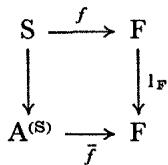
\includegraphics[keepaspectratio]{images/part003_a94682a2.jpg}}

(where the vertical arrow on the left is the canonical mapping \(s \mapsto e_s\) ).

Let \(\bar{f}:\mathbf{A}^{(\mathrm{S})}\to\mathbf{F}\) be the unique A-module homomorphism such that \(\bar{f}(e_{s})=\bar{f}(s)\) (II, §1, no. 11, Corollary 3 to Proposition 17); it suffices to verify that \(\bar{f}\) is an algebra homomorphism and for this it suffices to prove that \(\bar{f}(e_{s}e_{t})=\bar{f}(e_{s})\bar{f}(e_{t})\) , which follows immediately from the definition and the hypothesis \(f(st)=f(s)f(t)\) .

Proposition 6 expresses the fact that the ordered pair consisting of \(\mathbf{A}^{(\mathbb{S})}\) and the canonical mapping \(s\mapsto e_s\) is a solution of the universal mapping problem (Set Theory, IV, §3, no. 1) where \(\Sigma\) is the species of A-algebra structure and the \(\alpha\) -mappings the homomorphisms of S into an A-algebra with only its multiplicative law.

COROLLARY. Let S, S' be two magmas and \(g:S\to S'\) a homomorphism. Then there exists one and only one A-algebra homomorphism \(u:A^{(S)}\to A^{(S')}\) rendering commutative the diagram

\pandocbounded{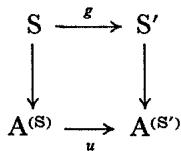
\includegraphics[keepaspectratio]{images/part003_71823134.jpg}}

(where the vertical arrows are the canonical mappings).

It suffices to apply Proposition 6 taking \(f\) to be the composite mapping \(\mathbf{S} \xrightarrow{g} \mathbf{S}' \to \mathbf{A}^{(\mathbf{S}')}\) .

In particular, if T is a stable subset of the magma S (I, § 1, no. 4), the set of elements \(\sum_{s\in\mathbf{T}}\alpha_s e_s\) of \(\mathbf{A}^{(\mathbf{S})}\) is a subalgebra of \(\mathbf{A}^{(\mathbf{S})}\) canonically isomorphic to the algebra \(\mathbf{A}^{(\mathbf{T})}\) and sometimes identified with the latter.

Example. Let V be an A-module and S a monoid which operates on V on the left; this means (I, § 5, no. 1) that there is given a mapping \((s, x) \mapsto s.x\) of S into V such that \(s.(x + y) = s.x + s.y\) , \(s.(\alpha x) = \alpha(s.x)\) and \(s.(t.x) = (st).x\) for \(s, t\) in S, \(x, y\) in V and \(\alpha \in \mathbf{A}\) and, denoting by \(e\) the identity element of S, e.x = x for \(x \in V\) . Writing \(f(s)(x) = s.x\) , f is a homomorphism of S into the algebra \(\operatorname{End}_{\mathbf{A}}(\mathbf{V})\) (with only its multiplicative law), mapping the identity element e to the unit element \(1_{V}\) . Applying Proposition 6, an A-algebra homomorphism \(\bar{f}: \mathbf{A}^{(\mathbf{S})} \to \operatorname{End}_{\mathbf{A}}(\mathbf{V})\) is obtained, which gives the underlying group of V a left module structure over \(\mathbf{A}^{(\mathbf{S})}\) .

This allows us to reduce the study of commutative groups with operators to that of modules. For let M be a commutative group with operators written additively, all of whose external laws are written multiplicatively. Let \(\Omega\) be the sum set (Set Theory, II, §4, no. 8) of the domains of operators of the various external laws on M, each of these domains being canonically identified with a subset of \(\Omega\) . Let \(\mathrm{Mo}(\Omega)\) be the free monoid (I §7, no. 2) constructed on \(\Omega\) ; a law of action

\[
(s, x) \mapsto s. x
\]

is defined on M with \(\mathrm{Mo}(\Omega)\) as domain of operators, by induction on the length of the word s in \(\mathrm{Mo}(\Omega)\) ; if s is of length 0, it is the empty word e and we write e.x = x for all \(x \in M\) . If x is of length \(n \geqslant 1\) , it can be written uniquely as s = tu, where u is of length n - 1 and t of length 1, so that \(t \in \Omega\) ; we then write s.x = t.(u.x). For any two words s, \(s'\) in \(\mathrm{Mo}(\Omega)\) , the relation \(s.(s'.x) = (ss').x\) is verified by induction on the length of s.

Then applying the method described above, a left \(\mathbf{Z}^{(\mathrm{Mo}(\Omega))}\) -module structure is obtained on M and it is verified without difficulty that the usual notions in the theory of groups with operators (stable subgroups, homomorphisms) are the same for commutative groups with operators and the modules thus associated with them.

\subsection{FREE ALGEBRAS}

DEFINITION 2. Let I be a set; let M(I) (resp. Mo(I), resp. N \(^{(I)}\) ) denote the free magma (resp. free monoid, resp. free commutative monoid) derived from I. The algebra of M(I) (resp. Mo(I), resp. N \(^{(I)}\) ) over A is called the free algebra (resp. free associative algebra, resp. free commutative associative algebra (or, by an abuse of language, free commutative algebra)) of the set I over the ring A.

We shall denote the free algebra (resp. free associative algebra, resp. free commutative algebra) of I over A by \(\operatorname{Lib}_{\mathbf{A}}(\mathbf{I})\) (resp. \(\operatorname{Libas}_{\mathbf{A}}(\mathbf{I})\) , resp. \(\operatorname{Libasc}_{\mathbf{A}}(\mathbf{I})\) ). By composing the canonical mapping of I into \(\operatorname{M}(\mathbf{I})\) (resp. \(\operatorname{Mo}(\mathbf{I})\) , resp. \(\mathbf{N}^{(\mathbf{I})}\) ) with the canonical mapping of \(\operatorname{M}(\mathbf{I})\) (resp. \(\operatorname{Mo}(\mathbf{I})\) , resp. \(\mathbf{N}^{(\mathbf{I})}\) ) into \(\operatorname{Lib}_{\mathbf{A}}(\mathbf{I})\) (resp. \(\operatorname{Libas}_{\mathbf{A}}(\mathbf{I})\) , resp. \(\operatorname{Libasc}_{\mathbf{A}}(\mathbf{I})\) ), a canonical mapping is obtained of I into \(\operatorname{Lib}_{\mathbf{A}}(\mathbf{I})\) (resp. \(\operatorname{Libas}_{\mathbf{A}}(\mathbf{I})\) , resp. \(\operatorname{Libasc}_{\mathbf{A}}(\mathbf{I})\) ), which is injective if \(A \neq \{0\}\) . We shall denote the image of an element \(i \in I\) under this canonical mapping by \(X_{i}\) and we shall say that \(X_{i}\) is the indeterminate of index i of \(\operatorname{Lib}_{\mathbf{A}}(\mathbf{I})\) (resp. \(\operatorname{Libas}_{\mathbf{A}}(\mathbf{I})\) , resp. \(\operatorname{Libasc}_{\mathbf{A}}(\mathbf{I})\) ).

As \(\mathbf{Mo}(\mathbf{I})\) and \(\mathbf{N}^{(\mathrm{I})}\) each have an identity element, \(\operatorname{Libas}_{\mathbf{A}}(\mathbf{I})\) and \(\operatorname{Libasc}_{\mathbf{A}}(\mathbf{I})\)

are unital associative algebras and further \(\operatorname{Libasc}_{\mathbf{A}}(\mathbf{I})\) is commutative. If e is the unit element of \(\operatorname{Libas}_{\mathbf{A}}(\mathbf{I})\) (resp. \(\operatorname{Libasc}_{\mathbf{A}}(\mathbf{I})\) ), the mapping \(\alpha \mapsto \alpha e\) is an isomorphism of A onto a subring of the centre of \(\operatorname{Libas}_{\mathbf{A}}(\mathbf{I})\) (resp. \(\operatorname{Libasc}_{\mathbf{A}}(\mathbf{I})\) ), which is identified with A (no. 1).

PROPOSITION 7. Let I be a set and F an algebra (resp. unital associative algebra, resp. unital commutative associative algebra) over A. For every mapping \(f:\mathbf{I}\to\mathbf{F}\) , there exists one and only one homomorphism (resp. unital homomorphism) \(\bar{f}\) of \(\operatorname{Lib}_{\mathbf{A}}(\mathbf{I})\) (resp. \(\operatorname{Libas}_{\mathbf{A}}(\mathbf{I})\) , resp. \(\operatorname{Libasc}_{\mathbf{A}}(\mathbf{I})\) ) into F such that \(\bar{f}(\mathbf{X}_{i})=f(i)\) for all \(i\in\mathbf{I}\) .

Let \(F_{m}\) be the magma (resp. monoid) obtained by giving the set F its multiplicative law of composition. There is one and only one homomorphism (resp. unital homomorphism) g of M(I) (resp. Mo(I), resp. N \(^{(I)}\) ) into \(F_{m}\) such that \(g(i) = f(i)\) for all \(i \in I\) (I, § 7, nos. 1, 2 and 7); Proposition 7 then follows from no. 6, Proposition 6.

Remarks. (1) We shall later define an isomorphism of \(\operatorname{Libas}_{\mathbf{A}}(\mathbf{I})\) onto the tensor algebra of the free module \(\mathbf{A}^{(I)}\) ( \(\S 5\) , no. 5) and also an isomorphism of \(\operatorname{Libasc}_{\mathbf{A}}(\mathbf{I})\) onto the symmetric algebra of \(\mathbf{A}^{(I)}\) ( \(\S 6\) , no. 6).

\begin{enumerate}
\def\labelenumi{(\arabic{enumi})}
\setcounter{enumi}{1}
\item
  Let \(\rho\) be a unital homomorphism of A into a commutative ring B. As has been seen (§ 2, no. 6), an isomorphism \(\sigma\) is derived from \(\rho\) of \(\operatorname{Lib}_{\mathbf{B}}(\mathbf{I})\) (resp. \(\operatorname{Libas}_{\mathbf{B}}(\mathbf{I})\) , resp. \(\operatorname{Libasc}_{\mathbf{B}}(\mathbf{I})\) ) onto the algebra \((\operatorname{Lib}_{\mathbf{A}}(\mathbf{I}))_{(\mathbf{B})}\) (resp. \((\operatorname{Libas}_{\mathbf{A}}(\mathbf{I}))_{(\mathbf{B})}\) , resp. \((\operatorname{Libasc}_{\mathbf{A}}(\mathbf{I}))_{(\mathbf{B})}\) ) obtained by extending the scalars to B by means of \(\rho\) ; if \(\mathbf{X}_i^{\mathbf{A}}\) , \(\mathbf{X}_i^{\mathbf{B}}\) are the indeterminates of index \(i\) corresponding respectively to A and B, then \(\sigma(\mathbf{X}_i^{\mathbf{B}}) = \mathbf{X}_i^{\mathbf{A}} \otimes 1\) .
\item
  Let \(J\) be a subset of \(I\) ; we know that \(M(J)\) is identified with a stable subset of the magma \(M(I)\) and hence (no. 6) \(\operatorname{Lib}_{A}(J)\) is canonically identified with a subalgebra of \(\operatorname{Lib}_{A}(I)\) , generated by the \(X_i\) such that \(i \in J\) ; it is said that only the indeterminates of indices belonging to \(J\) occur in an element of \(\operatorname{Lib}_{A}(J)\) . The definition given in no. 6 of the algebra of a magma shows that \(\operatorname{Lib}_{A}(I)\) is the union of the directed family of subalgebras \(\operatorname{Lib}_{A}(J)\) when \(J\) runs through the set of finite subsets of \(I\) . There are analogous results for \(\operatorname{Libas}_{A}(I)\) and \(\operatorname{Libasc}_{A}(I)\) .
\item
  With element \(s\) of \(\mathbf{M}(\mathbf{I})\) (resp. \(\mathbf{Mo}(\mathbf{I})\) , resp. \(\mathbf{N}^{(1)}\) ) is associated its length \(l(s)\) , which is an integer \(\geqslant 1\) (resp. \(\geqslant 0\) ) such that \(l(ss') = l(s) + l(s')\) (I, §7, nos. 1, 2 and 7). If \(e_s\) is the element of \(\operatorname{Lib}_{\mathbf{A}}(\mathbf{I})\) (resp. \(\operatorname{Libas}_{\mathbf{A}}(\mathbf{I})\) , resp. \(\operatorname{Libasc}_{\mathbf{A}}(\mathbf{I})\) ) corresponding to \(s\) , the total degree (or simply the degree of an element \(x = \sum_{s} \alpha_s e_s \neq 0\) of \(\operatorname{Lib}_{\mathbf{A}}(\mathbf{I})\) (resp. \(\operatorname{Libas}_{\mathbf{A}}(\mathbf{A})\) , resp. \(\operatorname{Libasc}_{\mathbf{A}}(\mathbf{I})\) ) is the greatest of the numbers \(l(s)\) when \(s\) runs through the (non-empty by hypothesis) set of elements such that \(\alpha_s \neq 0\) . For example, if \(i, j, k\) are three distinct elements of \(\mathbf{I}\) , the element \((\mathrm{X}_t(\mathrm{X}_j\mathrm{X}_k))\mathrm{X}_t - (\mathrm{X}_t\mathrm{X}_j)(\mathrm{X}_k\mathrm{X}_l)\) is an element \(\neq 0\) of total degree 4 in \(\operatorname{Lib}_{\mathbf{A}}(\mathbf{I})\) .
\end{enumerate}

\subsection{DEFINITION OF AN ALGEBRA BY GENERATORS AND RELATIONS}

Let \(\mathbf{F}\) be an algebra over \(\mathbf{A}\) and \((x_{i})_{i\in I}\) a family of elements of \(\mathbf{F}\) . By no. 7, Proposition 7, there exists a unique homomorphism \(f\colon \operatorname{Lib}_{\mathbf{A}}(\mathbf{I})\to \mathbf{F}\) such that \(f(\mathbf{X}_i) = x_i\) for all \(i\in I\) . For \(f\) to be surjective, it is necessary and sufficient that \((x_{i})_{i\in I}\) be a generating system of \(\mathbf{F}\) .

If \(\mathbf{U} \in \operatorname{Lib}_{\mathbf{A}}(\mathbf{I})\) , \(f(\mathbf{U})\) is called the element of \(\mathbf{F}\) derived from \(\mathbf{U}\) by substituting the elements \(x_{i}\) for the indeterminates \(\mathbf{X}_{i}\) , or also the value of \(\mathbf{U}\) for the values \(x_{i}\) of the indeterminates \(\mathbf{X}_{i}\) ; it is usually denoted by \(\mathbf{U}((x_{i})_{i \in I})\) ; in particular \(\mathbf{U}((\mathbf{X}_{i})_{i \in I}) = \mathbf{U}\) . If \(\lambda\) is a homomorphism of \(\mathbf{F}\) into an algebra \(\mathbf{F}'\) over \(\mathbf{A}\) , then

\[
\lambda (\mathrm{U} ((x _ {i}) _ {i \in \mathrm{I}})) = \mathrm{U} ((\lambda (x _ {i})) _ {i \in \mathrm{I}}).
\]

Consider in particular the case where \(\mathrm{F} = \operatorname{Lib}_{\mathbf{A}}(\mathbf{J})\) , where J is another set; for every family \((\mathrm{H}_{i})_{i \in I}\) of elements of \(\operatorname{Lib}_{\mathbf{A}}(\mathbf{J})\) and every family \((y_{j}')_{j \in J}\) of elements of an A-algebra \(F'\) ,

\[
\mathrm{U} ((\mathrm{H} _ {i}) _ {i \in I})) ((y _ {j} ^ {\prime}) _ {j \in J}) = \mathrm{U} ((\mathrm{H} _ {i} ((y _ {j} ^ {\prime}) _ {j \in J})) _ {i \in I}).\tag{37}
\]

In the above notation, every element U of \(\operatorname{Lib}_{\mathbf{A}}(\mathbf{I})\) such that \(\mathrm{U}((x_{i})_{i\in\mathbf{I}})=0\) , or also such that \(f(\mathrm{U})=0\) , is called a relator of the family \((x_{i})_{i\in\mathbf{I}}\) in F. The two-sided ideal \(\operatorname{Ker}(f)\) consisting of these elements is called the ideal of relators of \((x_{i})\) .

Let \((\mathbf{R}_j)_{j\in J}\) be a family of elements of \(\operatorname{Lib}_{\mathbf{A}}(\mathbf{I})\) . \(((x_i)_{i\in I}, (\mathbf{R}_j)_{j\in J})\) is called a presentation of the algebra \(F\) if \((x_i)_{i\in I}\) is a generating system of \(F\) and the two-sided ideal of \(\operatorname{Lib}_{\mathbf{A}}(\mathbf{I})\) generated by the \(\mathbf{R}_j\) is equal to the ideal of relators of the family \((x_i)_{i\in I}\) ; the \(x_i\) are called the generators and the \(\mathbf{R}_j\) the relators of the presentation.

Consider now any set I and a family \((\mathbf{R}_j)_{j\in J}\) of elements of \(\operatorname{Lib}_{\mathbf{A}}(\mathbf{I})\) . The quotient algebra E of \(\operatorname{Lib}_{\mathbf{A}}(\mathbf{I})\) by the two-sided ideal generated by the family \((\mathbf{R}_j)\) is called the universal algebra defined by the generating system I related by the family of relators \((\mathbf{R}_j)_{j\in J}\) . Clearly, if \(\overline{\mathbf{X}}_i\) denotes the image of \(\mathbf{X}_i\) in E,

\[
\left(\left(\overline {{\mathbf {X}}} _ {i}\right) _ {i \in I}, \left(\mathbf {R} _ {j}\right) _ {j \in J}\right)
\]

is a presentation of E. Moreover, if \((x_{i})_{i\in I}\) is a family of elements of an algebra F and \(\mathbf{R}_j((x_i)_{i\in I}) = 0\) for all \(j\in J\) , there exists a unique homomorphism \(g:\mathbf{E}\to \mathbf{F}\) such that \(g(\overline{\mathbf{X}}_i) = x_i\) for all \(i\in I\) ; for \(((x_i)_{i\in I},(\mathbf{R}_j)_{j\in J})\) to be a presentation of F, it is necessary and sufficient that \(g\) be bijective.

These remarks justify the following abuse of language: instead of saying `` \(((x_i)_{i \in I}, (R_j)_{j \in J})\) is a presentation of F'', it is also said that ``F is the algebra generated by the generators \(x_i\) subject to the relations \(R_j((x_i)_{i \in I}) = 0\) ''. When the \(R_j\) are of the form \(P_j - Q_j\) , it is also said that ``F is the algebra generated by the \(x_i\) subject to the relations \(P_j((x_i)) = Q_j((x_i))\) ''.

Let H be a set; we shall say that an element S of \(\operatorname{Lib}_{\mathbf{A}}(\mathbf{H})\) is a universal relator for an A-algebra F is \(\mathrm{S}((x_{h})_{h\in\mathbb{H}})=0\) for every family \((x_{h})_{h\in\mathbb{H}}\) of elements of F with H as indexing set.

Examples. (1) Take \(\mathbf{H} = \{1,2,3\}\) ; the algebras which admit

\[
(\mathrm{X} _ {1} \mathrm{X} _ {2}) \mathrm{X} _ {3} - \mathrm{X} _ {1} (\mathrm{X} _ {2} \mathrm{X} _ {3})
\]

as universal relator are the associative algebras. The algebras which admit \(X_{1}X_{2}-X_{2}X_{1}\) as universal relator are the commutative algebras. The algebras which admit the universal relators \(X_{1}X_{1}\) and

\[
(\mathrm{X} _ {1} \mathrm{X} _ {2}) \mathrm{X} _ {3} + (\mathrm{X} _ {2} \mathrm{X} _ {3}) \mathrm{X} _ {1} + (\mathrm{X} _ {3} \mathrm{X} _ {1}) \mathrm{X} _ {2}
\]

as universal relator are the Lie algebras.

Let I be a set; let a family \((\mathrm{S}_{k})_{k\in\mathbb{K}}\) of elements of \(\operatorname{Lib}_{\mathbf{A}}(\mathbf{H})\) be given and consider the set T of elements of \(\operatorname{Lib}_{\mathbf{A}}(\mathbf{I})\) of the form \(\mathrm{S}_{k}((\mathrm{U}_{h}))_{h\in\mathbb{H}}\) , where k runs through K and, for each \(k,\left(\mathrm{U}_{h}\right)_{h\in\mathbb{H}}\) runs through the set of families of elements of \(\operatorname{Lib}_{\mathbf{A}}(\mathbf{I})\) with H as indexing set; consider a family \((\mathrm{R}_{j})_{j\in\mathbb{J}}\) with T as set of elements. Then let F be the universal algebra defined by the generating system I related by the family \((\mathrm{R}_{j})_{j\in\mathbb{J}}\) and let \(u:\operatorname{Lib}_{\mathbf{A}}(\mathbf{I})\to\mathbf{F}\) be the canonical homomorphism, so that \(\operatorname{Ker}(u)\) is generated by the elements \(\mathrm{S}_{k}((\mathrm{U}_{h})_{h\in\mathbb{H}})\) for all \(k\in K\) and all families \((\mathrm{U}_{h})_{h\in\mathbb{H}}\) of elements of \(\operatorname{Lib}_{\mathbf{A}}(\mathbf{I})\) ; clearly each of the \(S_{k}\) \((k\in\mathbb{K})\) is a universal relator for F. Now let \(F'\) be an algebra admitting a generating system \((x_{i})_{i\in\mathbb{I}}\) , for which each of the \(S_{k}\) is a universal relator, and let \(u':\operatorname{Lib}_{\mathbf{A}}(\mathbf{I})\to\mathbf{F}'\) be the homomorphism such that \(u'(\mathrm{X}_{i})=x_{i}\) for all \(i\in I\) ; clearly \(\operatorname{Ker}(u)\subset\operatorname{Ker}(u')\) and hence \(u'\) can be written uniquely in the form \(u'=h\circ u\) , where \(h:F\to F'\) is a homomorphism such that \(h(\overline{\mathrm{X}}_{i})=x_{i}\) for all \(i\in I\) . For this reason F is called the universal algebra defined by the generating system I, corresponding to the family of universal relators \((\mathrm{S}_{k})_{k\in\mathbb{K}}\) . By an abuse of language, F is sometimes called the universal algebra generated by I and subject to the identities \(\mathrm{S}_{k}((u_{h}))=0\) for every family \((u_{h})_{h\in\mathbb{H}}\) of elements of F.

Example 2. Let \(\mathbf{L}'\) be the universal algebra generated by \(\mathbf{I}\) and subject to the identities \((uv)w - u(vw) = 0\) for every family of three elements of \(\mathbf{L}'\) and let \(\mathbf{L}''\) be the algebra obtained by adjoining a unit element to \(\mathbf{L}'\) ; then there exists a unique unital isomorphism \(g\) of \(\mathbf{L}''\) onto \(\operatorname{Libas}_{\mathbf{A}}(\mathbf{I})\) such that \(g(\overline{\mathbf{X}}_i) = \mathbf{X}_i\) for all \(i \in \mathbf{I}\) . For clearly \(\mathbf{L}''\) is associative and the existence of the homomorphism \(g\) follows from the definition of \(\mathbf{L}'\) and the remarks preceding it; but then clearly \(\mathbf{L}''\) satisfies the universal property (no. 7, Proposition 7) which characterizes \(\operatorname{Libas}_{\mathbf{A}}(\mathbf{I})\) , whence the conclusion.

Considerations analogous to the above can be applied to associative algebras (resp. commutative associative algebras), taking account of the following remarks. When the context gives sufficient indication that the algebras considered are unital algebras, by an abuse of language, a family of elements \((x_{i})_{i\in I}\) of an algebra \(F\) , such that the subalgebra generated by the \(x_{i}\) ( \(i\in I\) ) and the unit element is equal to \(F\) , is often called a generating system of \(F\) . Then let \(F\) be a unital associative algebra over \(A\) and let \((x_{i})_{i\in I}\) be a family of elements of \(F\) ; by virtue of no. 7, Proposition 7, there exists a unique unital homomorphism \(f:\mathrm{Libas}_{\mathbf{A}}(\mathbf{I})\to F\) such that \(f(\mathbf{X}_i) = x_i\) for all \(i\in I\) ; if \(\mathbf{U}\in \mathrm{Libas}_{\mathbf{A}}(\mathbf{I}), f(\mathbf{U})\) is also called the element of \(F\) derived from \(\mathbf{U}\) by substituting the elements \(x_{i}\) for the indeterminates \(\mathbf{X}_i\) and it is also denoted by \(\mathrm{U}((x_{i})_{i\in I})\) . Then the notions of relator, presentation and universal relator go over immediately to associative algebras; it suffices simply to replace \(\mathrm{Lib}_{\mathbf{A}}(\mathbf{I})\) throughout by \(\mathrm{Libas}_{\mathbf{A}}(\mathbf{I})\) . The universal unital associative algebra defined by the generating system \(I\) related by the family of relators \((\mathbb{R}_j)_{j\in J}\) is the quotient algebra of \(\mathrm{Libas}_{\mathbf{A}}(\mathbf{I})\) by the two-sided ideal generated by the family \((\mathbb{R}_j)\) . The universal unital associative algebra generated by the generating system \(I\) , corresponding to a family of universal relators is defined similarly. We leave to the reader the task of stating the analogous definitions relative to commutative associative algebras with \(\mathrm{Libasc}_{\mathbf{A}}(\mathbf{I})\) substituted for \(\mathrm{Libas}_{\mathbf{A}}(\mathbf{I})\) .

Example 3. Let L' be the universal unital associative algebra generated by I and subject to the identities uv - vu = 0 for every family of two elements of L'. It is seen, as in Example 2, that L' is canonically isomorphic to \(\text{Libasc}_{\mathbf{A}}(\mathbf{I})\) .

\subsection{POLYNOMIAL ALGEBRAS}

Let B be a unital commutative associative A-algebra and let \((x_{i})_{i\in I}\) be a family of elements of B; the subalgebra of B generated by the \(x_{i}\) ( \(i\in I\) ) and the unit element is denoted by \(\mathrm{A}[(x_{i})_{i\in I}]_{\mathrm{B}}\) or simply \(\mathrm{A}[(x_{i})_{i\in I}]\) when no confusion can arise. For every set I, the algebra \(\operatorname{Libasc}_{\mathbf{A}}(\mathbf{I})\) is therefore equal to \(\mathrm{A}[(\mathbf{X}_{i})_{i\in I}]\) (also denoted by \(\mathrm{A}[\mathbf{X}_{i}]_{i\in I}\) ); the latter notation, which has the advantage of indicating the notation chosen to denote the indeterminates, is the one we shall generally use in the rest of this Treatise. The elements of \(\mathrm{A}[(\mathbf{X}_{i})_{i\in I}]\) are called polynomials in the indeterminates \(X_{i}\) ( \(i\in I\) ) with coefficients in A; it is a convention that, when it is said ``let \(\mathrm{A}[(\mathbf{X}_{i})_{i\in I}]\) be a polynomial algebra'', the \(X_{i}\) are always understood to be the indeterminates. For every subset J of I, the use of the above notation amounts to identifying \(\operatorname{Libasc}_{\mathbf{A}}(\mathbf{J})\) with the algebra of \(\operatorname{Libasc}_{\mathbf{A}}(\mathbf{I})\) generated by the \(X_{i}\) of index \(i\in J\) and the unit element (cf.~no. 7, Remark (3)). For \(I=\{1,2,\ldots,n\}\) , we write \(\mathrm{A}[\mathbf{X}_{1},\mathbf{X}_{2},\ldots,\mathbf{X}_{n}]\) instead of \(\mathrm{A}[(\mathbf{X}_{i})_{i\in I}]\) .

If I and I' are two equipotent sets, the algebras \(\operatorname{Libasc}_{\mathbf{A}}(\mathbf{I})\) and \(\operatorname{Libasc}_{\mathbf{A}}(\mathbf{I}')\) are isomorphic. A{[}X{]} is often used to denote the polynomial algebra corresponding to an unspecified indexing set with a single element, X denoting the unique indeterminate; similarly, A{[}X, Y{]}, A{[}X, Y, Z{]}, \ldots{} are used to denote the polynomial algebras corresponding to unspecified indexing sets with

2, 3, \ldots{} elements. Note that, by virtue of the conventions made above, A{[}X{]} and A{[}Y{]} are for example (distinct) subalgebras of A{[}X, Y, Z{]} if A ≠ \{0\}.

The elements

\[
\mathrm{X} ^ {\nu} = \prod_ {i \in I} \mathrm{X} _ {i} ^ {\nu (i)},
\]

where v runs through \(\mathbf{N}^{(1)}\) form a basis of the polynomial algebra \(\mathrm{A}[(\mathrm{X}_{i})_{i\in\mathbb{I}}]\) . These elements are called monomials in the indeterminates \(X_{i}\) and the number \(|v|=\sum_{i\in\mathbb{I}}v(i)\) is called the degree (or total degree) of the monomial \(X^{v}\) . The unique monomial of degree 0 is the unit element of \(\mathrm{A}[(\mathrm{X}_{i})_{i\in\mathbb{I}}]\) ; it is often identified with the unit element 1 of A. Every polynomial u of \(\mathrm{A}[(\mathrm{X}_{i})_{i\in\mathbb{I}}]\) can be written uniquely as

\[
u = \sum_ {v \in \mathbf {N} ^ {(I)}} \alpha_ {v} X ^ {v}
\]

with \(\alpha_{\nu} \in \mathbf{A}\) ; the elements \(\alpha_{\nu}\) , zero except for a finite number of indices \(\nu \in \mathbf{N}^{(1)}\) , are called the coefficients of \(u\) ; the elements \(\alpha_{\nu} \mathrm{X}^{\nu}\) are called the terms of \(u\) (the element \(\alpha_{\nu} \mathrm{X}^{\nu}\) often being called the ``term in \(\mathrm{X}^{\nu''}\) ); in particular the term \(\alpha_{0} \mathrm{X}^{0}\) (identified with \(\alpha_{0} \in \mathbf{A}\) ) is called the constant term of \(u\) . If \(J\) is a subset of \(I\) , \(u\) belongs to \(\mathrm{A}[(\mathrm{X}_{i})_{i \in J}]\) if and only if \(\alpha_{\nu} = 0\) for \(\nu \notin \mathbf{N}^{(J)}\) . It follows that \(\mathrm{A}[(\mathrm{X}_{i})_{i \in I}]\) is the union of the subalgebras \(\mathrm{A}[(\mathrm{X}_{i})_{i \in J}]\) , where \(J\) runs through the set of finite subsets of \(I\) . If \(\alpha_{\nu} = 0\) for \(|\nu| > n\) , \(u\) is said to be a polynomial of degree \(\leqslant n\) . When \(\alpha_{\nu} = 0\) , (by an abuse of language) \(u\) is said to contain no term in \(\mathrm{X}^{\nu'}\) ; in particular, when \(\alpha_{0} = 0\) , \(u\) is said to be a polynomial with no constant term.

For every non-zero polynomial \(u = \sum_{v} \alpha_v X^v\) , the degree (or total degree) of \(u\) is the greatest of the integers \(|v|\) of the multiindices \(v\) such that \(\alpha_v \neq 0\) .

Let F be a unital associative A-algebra and let \((x_{i})_{i\in I}\) be a family of elements of F, which are pairwise permutable. The subalgebra \(F'\) of F generated by the \(x_{i}\) and the unit element is commutative (§1, no. 7), which allows us to define substituting the \(x_{i}\) for the \(X_{i}\) in the polynomial \(u\in\mathrm{A}[(X_{i})_{i\in I}]\) (although F is not necessarily commutative): \(u((x_{i})_{i\in I})\) is an element of \(F'\) and therefore of F and \(h\colon u\to u((x_{i})_{i\in I})\) is a homomorphism of \(\mathrm{A}[(X_{i})_{i\in I}]\) into F. The elements of the kernel of h are the relators of the family \((x_{i})\) in \(\mathrm{A}[(X_{i})_{i\in I}]\) , also called polynomial relators (with coefficients in A) between the \(x_{i}\) . The image of the homomorphism h is the subalgebra \(F'\) , also denoted by \(\mathrm{A}[(x_{i})_{i\in I}]\) (even when F is not commutative); if a is the ideal of polynomial relators between the \(x_{i}\) , then there is an exact sequence of A-modules

\[
0 \longrightarrow a \longrightarrow A [ (X _ {i}) _ {i \in I} ] \stackrel {h} {\longrightarrow} A [ (x _ {i}) _ {i \in I} ] \longrightarrow 0.
\]

PROPOSITION 8. Let \(\mathbf{A}[(\mathbf{X}_i)_{i\in I}]\) be a polynomial algebra, \(J\) a subset of \(I\) and \(K\) the complement of \(J\) in \(I\) . Writing \(\mathbf{A}' = \mathbf{A}[(\mathbf{X}_j)_{j\in J}]\) and denoting by \(\mathbf{X}_k'\) ( \(k\in K\) ) the indeterminates in the polynomial algebra \(\operatorname{Libasc}_{\mathbf{A}'}(\mathbf{K}) = \mathbf{A}'[(\mathbf{X}_k')_{k \in \mathbb{K}}]\) , there exists a unique ring isomorphism of \(\mathbf{A}'[(\mathbf{X}_k')_{k \in \mathbb{K}}]\) onto \(\mathbf{A}[(\mathbf{X}_i)_{i \in I}]\) which coincides with the identity on \(\mathbf{A}'\) and maps \(\mathbf{X}_k'\) to \(\mathbf{X}_k\) for all \(k \in \mathbb{K}\) .

Clearly \(\mathbf{A}[(\mathbf{X}_i)_{i\in I}]\) is an \(\mathbf{A}'\) -algebra generated by the \(\mathbf{X}_k\) for \(k\in \mathbf{K}\) . On the other hand, as a polynomial relator between the \(\mathbf{X}_k\) ( \(k\in \mathbf{K}\) ) with coefficients in \(\mathbf{A}'\) can be written uniquely as \(\sum_{\nu}h_{\nu}((\mathbf{X}_j)_{j\in J})\mathbf{X}^{\nu}\) where \(\nu\) runs through a finite subset of \(\mathbf{N}^{(\mathbb{R})}\) and where the \(h_\nu\) are elements of \(\mathbf{A}[(\mathbf{X}_j)_{j\in J}]\) , the \(h_\nu\) must be polynomial relators between the \(\mathbf{X}_j\) with coefficients in \(\mathbf{A}\) and hence are all zero, which proves the proposition.

The isomorphism described in Proposition 8 is often used to identify the elements of \(\mathbf{A}[(\mathbf{X}_i)_{i\in I}]\) with polynomials with coefficients in \(\mathbf{A}' = \mathbf{A}[(\mathbf{X}_j)_{j\in J}]\) . If \(u\) is an element \(\neq 0\) of \(\mathbf{A}[(\mathbf{X}_i)_{i\in I}]\) , its total degree considered as an element of \(\mathbf{A}'[(\mathbf{X}_k)_{k\in K}]\) is also called its degree with respect to the \(\mathbf{X}_i\) of index \(i\in K\) .

Remark. Let I and J be two sets and \((\mathrm{P}_{j})_{j\in J}\) a family of elements of \(\mathbf{Z}[(\mathrm{X}_{i})_{i\in I}]\) ; if Q is an element of \(\mathbf{Z}[(\mathrm{X}_{j})_{j\in J}]\) such that \(\mathbf{Q}((\mathrm{P}_{j})_{j\in J})=0\) , then, for every family \((b_{i})_{i\in I}\) of pairwise permutable elements of a ring B,

\[
\mathrm{Q} ((\mathrm{P} _ {j} ((b _ {i}) _ {i \in \mathrm{I}})) _ {j \in \mathrm{J}}) = 0.
\]

The relations which hold of the form \(\mathbf{Q}((\mathbf{P}_{j})_{j\in\mathbf{J}})=0\) are sometimes called polynomial identities. For example

\[
\left(\mathrm{X} _ {1} + \mathrm{X} _ {2}\right) ^ {2} - \mathrm{X} _ {1} ^ {2} - \mathrm{X} _ {2} ^ {2} - 2 \mathrm{X} _ {1} \mathrm{X} _ {2} = 0
\]

with

\[
\begin{array}{r l} \mathrm{Q} & = \mathrm{Y} _ {1} ^ {2} - \mathrm{Y} _ {2}, \qquad \mathrm{P} _ {1} = \mathrm{X} _ {1} + \mathrm{X} _ {2}, \qquad \mathrm{P} _ {2} = \mathrm{X} _ {1} ^ {2} + \mathrm{X} _ {2} ^ {2} + 2 \mathrm{X} _ {1} \mathrm{X} _ {2} \\ & \quad \mathrm{X} _ {1} ^ {n} - \mathrm{X} _ {2} ^ {n} - (\mathrm{X} _ {1} - \mathrm{X} _ {2}) (\mathrm{X} _ {1} ^ {n - 1} + \mathrm{X} _ {1} ^ {n - 2} \mathrm{X} _ {2} + \dots + \mathrm{X} _ {2} ^ {n - 1}) = 0 \end{array}
\]

with

\[
\begin{array}{c} \mathrm{Q} = \mathrm{Y} _ {1} - \mathrm{Y} _ {2} \mathrm{Y} _ {3}, \qquad \mathrm{P} _ {1} = \mathrm{X} _ {1} ^ {n} - \mathrm{X} _ {2} ^ {n}, \qquad \mathrm{P} _ {2} = \mathrm{X} _ {1} - \mathrm{X} _ {2}, \\ \mathrm{P} _ {3} = \mathrm{X} _ {1} ^ {n - 1} + \mathrm{X} _ {1} ^ {n - 2} \mathrm{X} _ {2} + \dots + \mathrm{X} _ {2} ^ {n - 1} \end{array}
\]

are polynomial identities.

\subsection{TOTAL ALGEBRA OF A MONOID}

The algebra of a monoid S over A is (as an A-module) the submodule of the product \(A^{s}\) consisting of the families \((\alpha_{s})_{s\in\mathbb{S}}\) of finite support; the multiplication in this algebra is defined by the relations \((\alpha_{s})(\beta_{s})=(\gamma_{s})\) , where, for all \(s\in S\) ,

\[
\gamma_ {s} = \sum_ {t u = s} \alpha_ {t} \beta_ {u}\tag{38}
\]

(cf.~no. 6, formula (35)). The sum on the right hand side of (38) is meaningful because \((\alpha_{s})\) and \((\beta_{s})\) are families of finite support and so therefore is the double family \((\alpha_{t}\beta_{u})_{(t,u)\in S\times S}\) . But the right hand side of (38) is also meaningful for arbitrary elements \((\alpha_{s})\) , \(\beta_{s})\) of \(A^{S}\) when the monoid \(S\) satisfies the following condition:

\begin{enumerate}
\def\labelenumi{(\Alph{enumi})}
\setcounter{enumi}{3}
\tightlist
\item
  For all \(s \in \mathbf{S}\) , there exists only a finite number of ordered pairs \((t, u)\) in \(\mathbf{S} \times \mathbf{S}\) such that \(tu = s\) .
\end{enumerate}

Suppose then that S satisfies condition (D); a multiplication law can then be defined on the product A-module \(A^{s}\) by formula (38). It is immediate that the multiplication thus defined on \(A^{s}\) is A-bilinear; also it is associative, since, for \(\alpha\) , \(\beta\) , \(\gamma\) in \(A^{s}\) ,

\[
\sum_ {u v w = t} \alpha_ {u} \beta_ {v} \gamma_ {w} = \sum_ {r w = t} \left(\left(\sum_ {u v = r} \alpha_ {u} \beta_ {v}\right) \gamma_ {w}\right) = \sum_ {u s = t} \left(\alpha_ {u} \left(\sum_ {v w = s} \beta_ {v} \gamma_ {w}\right)\right).
\]

This multiplication and the A-module structure on \(A^{s}\) therefore define on \(A^{s}\) a unital associative algebra structure over A; we shall say that the set \(A^{s}\) , with this structure, is the total algebra of the monoid S over A.

It is immediate that the algebra \(\mathbf{A}^{(\mathbf{S})}\) of the monoid \(\mathbf{S}\) over \(\mathbf{A}\) (also called the restricted algebra of \(\mathbf{S}\) when necessary to avoid confusion) is a subalgebra of the total algebra of \(\mathbf{S}\) over \(\mathbf{A}\) (and is identical with the latter when \(\mathbf{S}\) is finite). By an abuse of language, every element \((\xi_s)_{s \in \mathbf{S}}\) of the total algebra of \(\mathbf{S}\) over \(\mathbf{A}\) is also denoted by the same notation \(\sum_{s \in \mathbf{S}} \xi_s e_s\) (or even \(\sum_{s \in \mathbf{S}} \xi_s s\) ) as the elements of the restricted algebra of \(\mathbf{S}\) ; of course the summation symbol appearing in this notation corresponds to no algebraic operation because it is taken over an infinity of terms \(\neq 0\) in general. With this notation, multiplication in the total algebra of \(\mathbf{S}\) is also given by formula (35) of no. 6.

If S is commutative, so is its total algebra \(A^{S}\) . If T is a submonoid of S, the total algebra \(A^{T}\) of the monoid is canonically identified with a subalgebra of the total algebra of S. If \(\rho: A \to B\) is a ring homomorphism, the canonical extension \(\rho^{S}: A^{S} \to B^{S}\) is an A-homomorphism of the total algebra of S over A into the total algebra of S over B, which extends the canonical homomorphism \(A^{(S)} \to B^{(S)}\) .
